%% 
%% Copyright 2007-2024 Elsevier Ltd
%% 
%% This file is part of the 'Elsarticle Bundle'.
%% ---------------------------------------------
%% 
%% It may be distributed under the conditions of the LaTeX Project Public
%% License, either version 1.3 of this license or (at your option) any
%% later version.  The latest version of this license is in
%%    http://www.latex-project.org/lppl.txt
%% and version 1.3 or later is part of all distributions of LaTeX
%% version 1999/12/01 or later.
%% 
%% The list of all files belonging to the 'Elsarticle Bundle' is
%% given in the file `manifest.txt'.
%% 
%% Template article for Elsevier's document class `elsarticle'
%% with harvard style bibliographic references

\documentclass[preprint,12pt,authoryear]{elsarticle}

%% Use the option review to obtain double line spacing
%% \documentclass[authoryear,preprint,review,12pt]{elsarticle}

%% Use the options 1p,twocolumn; 3p; 3p,twocolumn; 5p; or 5p,twocolumn
%% for a journal layout:
%% \documentclass[final,1p,times,authoryear]{elsarticle}
%% \documentclass[final,1p,times,twocolumn,authoryear]{elsarticle}
%% \documentclass[final,3p,times,authoryear]{elsarticle}
%% \documentclass[final,3p,times,twocolumn,authoryear]{elsarticle}
%% \documentclass[final,5p,times,authoryear]{elsarticle}
%% \documentclass[final,5p,times,twocolumn,authoryear]{elsarticle}

%% For including figures, graphicx.sty has been loaded in
%% elsarticle.cls. If you prefer to use the old commands
%% please give \usepackage{epsfig}

%% The amssymb package provides various useful mathematical symbols
\usepackage{amssymb}
%% The amsmath package provides various useful equation environments.
\usepackage{amsmath}
%% The amsthm package provides extended theorem environments
%% \usepackage{amsthm}

%% The lineno packages adds line numbers. Start line numbering with
%% \begin{linenumbers}, end it with \end{linenumbers}. Or switch it on
%% for the whole article with \linenumbers.
%% \usepackage{lineno}

\usepackage{url}
\usepackage{xcolor}
\usepackage{subcaption}

\journal{European Journal of Operational Research}

\begin{document}

\begin{frontmatter}

%% Title, authors and addresses

%% use the tnoteref command within \title for footnotes;
%% use the tnotetext command for theassociated footnote;
%% use the fnref command within \author or \affiliation for footnotes;
%% use the fntext command for theassociated footnote;
%% use the corref command within \author for corresponding author footnotes;
%% use the cortext command for theassociated footnote;
%% use the ead command for the email address,
%% and the form \ead[url] for the home page:
%% \title{Title\tnoteref{label1}}
%% \tnotetext[label1]{}
%% \author{Name\corref{cor1}\fnref{label2}}
%% \ead{email address}
%% \ead[url]{home page}
%% \fntext[label2]{}
%% \cortext[cor1]{}
%% \affiliation{organization={},
%%            addressline={}, 
%%            city={},
%%            postcode={}, 
%%            state={},
%%            country={}}
%% \fntext[label3]{}

\title{The Truck-to-dock Door Assignment Problem: \\ analysis and discussion of IP formulations} %% Article title

%% use optional labels to link authors explicitly to addresses:
%% \author[label1,label2]{}
%% \affiliation[label1]{organization={},
%%             addressline={},
%%             city={},
%%             postcode={},
%%             state={},
%%             country={}}
%%
%% \affiliation[label2]{organization={},
%%             addressline={},
%%             city={},
%%             postcode={},
%%             state={},
%%             country={}}

\author[label1]{Nicolas Forget} %% Author name
  \ead{Nicolas.Forget@jku.at}
\author[label2]{Elizabeth Gandibleux} %% Author name
  \ead{Elizabeth.Gandibleux@etu.univ-nantes.fr}
\author[label2]{Xavier Gandibleux\corref{cor1}} %% Author name
  \ead{Xavier.Gandibleux@univ-nantes.fr}
\author[label2]{Valentin Guy--Deroubaix} %% Author name
  \ead{valentin.Guy-Deroubaix@etu.univ-nantes.fr}
\author[label2]{Awen Jacq--Bodet} %% Author name
  \ead{Awen.Jacq--Bodet@etu.univ-nantes.fr}

%% Author affiliation

\affiliation[label1]{organization={Johannes Kelper University Linz}, %Department and Organization
            addressline={Altenberger Straße 69}, 
            city={Linz},
            postcode={4040}, 
            country={Austria}}        
            
\affiliation[label2]{organization={Nantes University},%{Nantes Universit\'e}, %Department and Organization
            addressline={2, rue de la Houssiniere BP 92208}, 
            city={Nantes},
            postcode={44322 Cedex 03}, 
            country={France}}                

\cortext[cor1]{Corresponding author}

%
% =======================================================================
% =======================================================================
%

%% Abstract
\begin{abstract}
%% Text of abstract
This paper is devoted to (résumé posé à adapter)... %the Truck-to-dock Door Assignment Problem (TDAP), which is an optimisation problem in logistics and supply chain management, particularly in cross-docking centers.
%
%We present a thorough analysis of the state-of-the-art contributions on the TDAP that are in the continuation of the seminal work of \citet{MIAO2009}. 
%%
%Our contributions focus on the proposed mixed integer programming formulations, the datasets used and the exact solutions obtained.
%%
%We discuss the known limitations and others we have found in the scientific literature regarding two formulations. We correct errors, inaccuracies and incompleteness we identified.
%%
%We propose a revised single-objective formulation and a new dataset designed to more realistically reflect real-world exploitation. A numerical experiment on the three formulations discussed, with regard to the two classes of numerical instances named ``full mesh'' and``bi-partite'', is reported.
%%
%We also propose a bi-objective formulation whose resolution with generic algorithm is analysed and discussed. A numerical experiment comparing the exact solutions of the single-objective model and the bi-objective model gives the advantage to the latter for the quality of the solutions produced.
%%
%The produced codes are implemented in Julia, the mathematical formulations are written with JuMP, the MIP resolutions are made with the Gurobi solver. 
\end{abstract}

%
% =======================================================================
% =======================================================================
%

%%Graphical abstract
\begin{graphicalabstract}
%\includegraphics{grabs}
\end{graphicalabstract}

%
% =======================================================================
% =======================================================================
%

%%Research highlights
\begin{highlights}
\item Research highlight 1
\item Research highlight 2
\end{highlights}

%
% =======================================================================
% =======================================================================
%

%% Keywords
\begin{keyword}
%% keywords here, in the form: keyword \sep keyword

%% PACS codes here, in the form: \PACS code \sep code

%% MSC codes here, in the form: \MSC code \sep code
%% or \MSC[2008] code \sep code (2000 is the default)

Supply Chain Management \sep
Cross Docking \sep
Truck-to-dock Door Assignment Problem \sep 
Integer Programming Formulations\sep
Multi-objective Optimization
\end{keyword}

\end{frontmatter}

%% Add \usepackage{lineno} before \begin{document} and uncomment 
%% following line to enable line numbers
%% \linenumbers

%% main text
%%

\newpage
%
% =======================================================================
% =======================================================================
%
\section{Introduction} 
\label{sec:introduction}

%
% =======================================================================
%

\subsection{Background} % Context ?
\label{sec:Background}

In the context of supply chain operations, this paper addresses an operational  problem encountered in a cross-docking warehouse. 
%
Cross-docking is a logistics technique that aims to accelerate goods delivery and increase supply chain efficiency. 
%
Considering a warehouse with a given shape, the term cross-docking expresses the process of receiving products on inbound dock doors and then transferring them directly across the cross-dock to outbound dock doors, with few or no storage time in between (see Figure~\ref{fig:CrossDockVanBelle}).
%
\begin{figure}[h]
\begin{center}
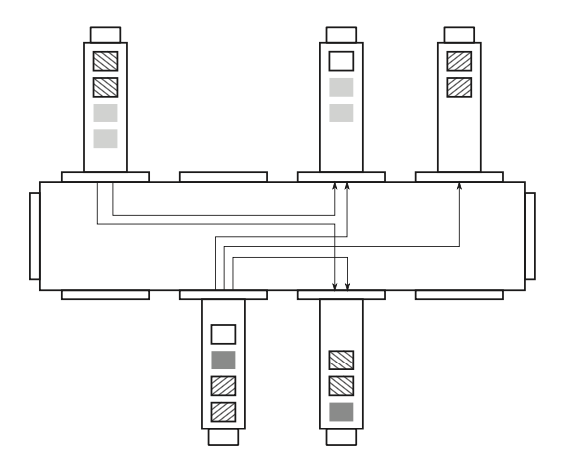
\includegraphics[scale=0.3]{images/CDvanBelle.png}
\caption{Illustration from \cite{VANBELLE2012} of a cross-dock where the layout of the warehouse presents a I-shape. Ten docks are available (flat rectangles) to serve as inbound or outbound of products. 
Five trucks are docked (long rectangles). 
A pallet of a given product is represented by a rectangle with a given pattern.
Each truck may convoy pallets of different products (represented by rectangles with different patterns).
Pallets are moved into the warehouse (represented by arrows) from inbound to outbound docks.}
\label{fig:CrossDockVanBelle}
\end{center}
\end{figure}
%
More precisely, incoming products arrive through means of transportation such as trucks, and are docked on inbound dock doors of the cross-dock terminal. Once incoming trucks have been docked, the pallets get unloaded, sorted and screened to identify their end destinations. 
%
Afterward, the pallets are moved to outbound dock doors of cross-dock terminal using e.g. material handling devices such as forklifts.

Cross-docking requires close coordination among a company’s supply chain partners, including its suppliers and freight carriers. According \citet{DefCrossDock2023}, this effort often pays off in multiple ways: companies can deliver products faster, minimize the need for warehouse space, optimize inventory control, and reduce transportation and labor costs.

Depending on the horizon of decisions considered (long term, mid term, short-term decisions)
the literature presents several decision problems related to cross-docking (see e.g \citet{VANBELLE2012,Nduwayo2020PhD} ). They are grouped in strategic (e.g. location of cross-docks and layout design),  tactical (e.g. cross-docking networks), and operational (e.g. vehicle routing, dock door assignment, truck scheduling and temporary storage) decision problems.

%
% =======================================================================
%
\subsection{The Truck-to-dock Door Assignment Problem}
\label{sec:TDAP}

In the context of cross-docking operations, the specific situation tackled is as follows: given a cross-dock warehouse composed of docks, and a planning of trucks where each truck is characterised by an arrival time, a departure time, and a number of pallets to transfert between trucks, the goal is to maximise the number of pallets transfered, and to minimize the time required to perform the operations. 
%a truck door assignment problem with time window constraints.
%
This statement leads to an assignment subproblem. Indeed,  when an inbound or outbound truck arrives at the cross-dock, it has to be decided to which dock door the truck should be assigned. A good assignment can increase the productivity of the cross-dock and can decrease the handling costs. 
%The dock door assignment problem tries to find the optimal assignment of inbound and outbound trucks to dock doors. 
Also, this statement leads to a scheduling subproblem.  Effectively, the dock doors are considered as resources (used by the trucks) that have to be scheduled over time. The problem decides on the succession of inbound and outbound trucks at the dock doors of a cross-dock: in a short, where and when should the trucks be processed.
%
Thus a model describing this optimization problem must take into account at minima  (1)~the arrival and departure of trucks, (2) the assignment of trucks to the docks, (3) the operational time for pallet shipment among the docks, and (4) the maximum amount of pallets that the crossdock can support.
\medskip

%
This optimization problem falls in the class of truck scheduling problem which deal with short-term decisions (operational). 
%
Among truck scheduling problems, those where scheduling of inbound and outbound trucks is the central problem are referred to as the \textit{Truck-to-dock Door Assignment Problem (TDAP)} in the literature. 
%
It is a combinatorial optimisation problem known to belong to the class of $\mathcal{NP}$-hard problems \citep{MIAO2009}.
% 
On the basis of the contributions of \citet{Lim2005,Lim2006,MIAO2009}, the TDAP is the optimization problem addressed in this paper, and the model introduced in \citet{MIAO2009} is our starting reference.

\medskip

In the literature, the various studies related to the TDAP consider different assumptions and settings, for instance regarding the preemption (allowed or not), the processing time to load or unload a truck (fixed or not for all trucks), intermediate storage (allowed or not), etc. In the following, we consider the case 
(1) without preemption (loading/unloading operations cannot be interrupted and resumed at a later time), and
(2) the processing time to load/unload trucks is fixed for all trucks.
The case with/without intermediate storage is discussed in this paper.


%
% =======================================================================
%
\subsection{Literature Review} 
\label{subsec:LiteratureReview}

%    Our bibliographic study has provided us an overview of the scientific literature published until 2021.

     \citet{MIAO2009} have extended a truck scheduling problem previously proposed by \cite{Lim2005,Lim2006} in which it is assumed that the trucks are loaded or unloaded during a fixed time window.
    This means that the optimization problem is reduced to determining at which dock door the trucks have to be processed. 
    The length of these time windows can be interpreted as the time needed to load or unload a truck. 
    %
    The trucks can be assigned to any door and the capacity of the cross-dock is limited. 
    Preemption is not allowed and trucks that cannot be served are
    penalized. 
    The objective here is to minimize the operational cost (based on travel time) plus the cost of unfulfilled shipments. 
    The authors formulate the problem with an Integer Programming (IP) model.     
    %
    This formulation is denoted ``formulation M'' in the remaining of the paper. 
    %
    Numerical experiments are reporting using CPLEX. 
    %
    Observing that CPLEX faces resolution difficulties, they have also proposed a tabu search and a genetic algorithm approach to solve it.


%--------------------------------------------------------------------------------------
    
    \citet{VANBELLE2012} present a vast state-of-the-art of the cross-docking concept. 
    First, the authors discuss on guidelines for the use and implementation of cross-docking.
    They describe characteristics that can be helpful to distinguish the different cross-dock types and provide an extensive  review of the existing literature until 2012 on cross-docking.
    %
    The papers discussed are classified based on the problem type tackled (e.g. internal transport type, temporary storage allowed or not, etc.), and promizing directions to improve and extend the contributions are suggested.

    % --------------------------------------------------------------------------------------

    Several  PhD thesis (e.g. \citet{Zhu2007PhD,Ladier2014PhD,Zhang2016PhD,Nassief2017PhD,Nduwayo2020PhD}) are devoted to decision problems related to cross-docking.
    For example, Nduwayo's contributions \citep{Nduwayo2020,Nduwayo2020PhD} are devoted to the ``Cross-Docking Assignment Problem (CDAP)'', i.e. the problem to assign origins to inbound doors and destinations to outbound doors so that the total cost inside the cross-dock platform is minimized (see e.g. \citet{TSUI1992,Zhu2009} or recently \citet{Belen2024}). Nduwayo proposes original Mixed-Integer Programming models, and he conductes an extensive comparative analysis on benchmark instances from the literature.

    % --------------------------------------------------------------------------------------    


     \citet{Gelareh2015} underline in a technical report available online  weaknesses and shortcomings in the formulation M. On the basis of the latter, they propose a revised IP formulation for the TDAP denoted ``formulation G'' in the rest of the paper.
    %
    Several classes of valid inequalities are also introduced, and exact separation algorithms are described for separating cuts for classes with exponential number of constraints. An efficient branch-and-cut algorithm solving real-life size instances in a reasonable time is provided.
    %
    Numerical experiments show that in most cases, the optimal solution is identified at the root node without requiring any branching.
    %
    The main contents of this report have been published in \cite{GELAREH2016}.
        
% --------------------------------------------------------------------------------------

    \citet{Kucukoglu2017} consider a variant of TDAP  with product placement plans.
    %
    To solve this problem, they propose a IP model where the objective is to find the truck-door assignment and product placement plans that minimize total travelling distance of the products.
    
    % --------------------------------------------------------------------------------------

    \citet{Daquin2021} have published recently  a paper devoted to the TDAP where the algorithms presented are based on the Variable Neighborhood Search metaheuristic. 
    %
    However, this work is based on the formulation~M, which is pointed out as incorrect since 2015 by  \citet{Gelareh2015}.
    %
    Thus, an another paper \citep{Gelareh2021} which refers to \citep{Gelareh2015,GELAREH2016} has been published which criticizes \cite{Daquin2021} and recalls the shortcomings already discussed about the formulation M.
    
    

%
% =======================================================================
%
\subsection{Contributions and Organisation of the Paper}

Given the points of contention observed along the literature review,  a careful reading of the four documents concerned  \citep{MIAO2009,Gelareh2015,GELAREH2016,Gelareh2021} has been achieved. 
    %
It has revealed inconsistencies in the arguments put forward in \citep{Gelareh2015,GELAREH2016,Gelareh2021}, as well as to observe several vagueness and incompleteness in the formulation G.
In particular,  the proposed  amendments in \citep{Gelareh2021} does not address accurately all  deficiencies raised in the formulation M, and the numerical results provided in \citep{GELAREH2016} are not replicable. 

On base of these four scientific documents questioned on several aspects, the first contribution of this paper is devoted to an analysis and a discussion of the M and G formulations and the optimal solutions obtained by them, aiming to provide to the readers 
(1)~an advanced understanding of the formulations, 
(2)~a corrected formulation of G, and 
(3)~an understanding of the optimal solutions collected with the two formulations.
Also,  an alternative formulation derived from G and considered less simplifying assumptions in the operations, named 2R, is proposed.
%
2R is a a bi-objective variant where 
(1) one constraint of G is modified and 
(2) the formulation's abilities to simultaneously optimize independently the two conflicting objectives is explored.

The second contribution of this paper concerns numerical experiments conducted with these formulations.
%
\citet{MIAO2009} describe the characteristics used for creating numerical instances generated to evaluate the algorithms proposed in their paper, but the corresponding datafiles are not provided.
%
\citet{GELAREH2016}  have generated datafiles  according the indications provided in \citep{MIAO2009} for evaluating their algorithms. They are available online.
%
We refer to these instances in the following as ``full mesh'' instances.
%
In addition, a new set of numerical instances inspired from a real crossdock warehouse and plannings of trucks where the management of pallets is more realistic have been generated.
These instances will be referred to in the following as ``bipartite'' instances.
%
Numerical experiments have been conducted using these two distinct sets of instances, allowing the evaluation of the formulation's performance across various scenarios.

The rest of the paper is organised as follow.
%
Section~\ref{sec:Notations} presents  the notations and the definitions of the parameters. 
In order to facilitate the discussions about formulations,  the notations used for the formulations have been unified.
Next, an illustrating example based on a toy instance is used to review the different values that  parameters may take, and the type of solution returned.
%
Formulation M is presented in Section~\ref{sec:FormulationM}, followed by criticism found in the literature in Section~\ref{sec:discussionM}.
%
Next, formulations G and 2R are respectively introduced in Section~\ref{sec:FormulationG} and Section~\ref{sec:Formulation2R}.
The three formulations are rigorously described, and come with a comments and a discussion.
%
Numerical experiments are reported in Section~\ref{sec:NumericalExperiments}. The two sets of instances are presented and the results collected are reported and analysed.
%
Finally, Section~\ref{sec:ConclusionPerspectives} gives a conclusion and draws several perspectives.
%
The formulations are implemented in Julia \citep{Julia2017} with JuMP \citep{JuMP2023}, and they are provided in \ref{app:formulations}. 
Also, in order to allow the readers to reproduce all results presented in this paper, all the material produced, i.e. codes in Julia, formulations in JuMP, and datasets in raw text files, are available online on GitHub at \url{https://github.com/xgandibleux/TDAP}.

\newpage
%
% =======================================================================
% =======================================================================
%
\section{Notations, Parameters, Example} 
\label{sec:Notations}


%
% =======================================================================
%

\subsection{Parameters}
\medskip

\noindent
The following parameters are used in the formulations: 
\begin{itemize}
    \item []$N$: \hspace{1.5mm}set of trucks arriving at and/or departing from the crossdock
    \item []$M$: \hspace{1.1mm}set of docks available in the crossdock
    \item []$n$: \hspace{2.5mm}total number of trucks, that is $|N|$ %(where $|N|$ denotes the cardinality of $N$)
    \item []$m$: \hspace{1.5mm}total number of docks, that is $|M|$ 
    \item []$a_i$: \hspace{1.5mm}arrival time of truck $i$ \hfill$(1 \leq i \leq n)$
    \item []$d_i$: \hspace{1.5mm}departure time of truck $i$ \hfill$(1 \leq i \leq n)$
    \item []$t_{kl}$: \hspace{1mm}operational time for pallets from dock $k$ to dock $l$ \hfill $(1 \leq k,l \leq m)$
    \item []$f_{ij}$: \hspace{1mm}number of pallets transferring from truck $i$ to truck $j$ \hfill$(1 \leq i,j \leq n)$
    \item []$c_{kl}$: \hspace{1mm}operational cost per unit time from dock $k$ to dock $l$ \hfill$(1 \leq k,l \leq m)$
    \item []$p_{ij}$: \hspace{1mm}penalty cost per unit cargo from truck $i$ to truck $j$ \hfill$(1 \leq i,j \leq n)$
    \item []$C$: \hspace{2mm}capacity of crossdock
    \item []$\hat{x}_{ij}$: \hspace{0.5mm}1 iff truck $i$ departs no later than truck $j$ arrives; 0 otherwise
\end{itemize}
\medskip

\noindent
It is reasonable and no restrictive to adopt the following considerations:
\begin{enumerate}
    \item $f_{ij} \geq  0$ iff $d_{j} \geq a_{i}$ $(1 \leq i,j \leq n)$, otherwise $f_{ij} = 0$ \\
    It means that truck $i$ will transfer some cargo to truck $j$ iff truck $j$ departs no earlier than truck $i$ arrives;
    
    \item $a_{i} < d_i$ $(1 \leq i \leq n)$\\
    It means that for each truck, the arrival time should strictly smaller than its departure time;
    
    \item $n > m$\\ 
    It considers the over-constrained condition.
\end{enumerate}
\medskip

\noindent
In order to facilitate the expression of the set of capacity constraints, a vector of data named $\tau$ 
is built from $a_{i}$ and $d_{i}$ as follows:


    \begin{enumerate}
        \item sort all $a_{i}$ and $d_{i}$ in an increasing order;
        \item let $\tau_r$ 
        $(r = 1, 2, ..., 2n)$ be these $2n$ numbers such that $\tau_{1} \leq \tau_{2} \leq ... \leq \tau_{2n}$.
    \end{enumerate}    

%
% =======================================================================
%
\subsection{Illustrative Example}
Let's take a toy example illustrated by Figure \ref{fig:Example1}, which shows the parameters to handle:
%\vspace{-3mm}
    \begin{figure}[h!]
    \begin{subfigure}{0.425\textwidth}
    \centering
      \includegraphics[scale=0.11]{images/exemple1Crossdock.png} 
      \caption{The layout of the crossdock. Values on arrows report the transfert time $t_{kl}$ between docks $k$ and $l$.}
      \label{fig:layoutexample}
    \end{subfigure}
    \hfill
    \begin{subfigure}{0.525\textwidth}
    \centering
      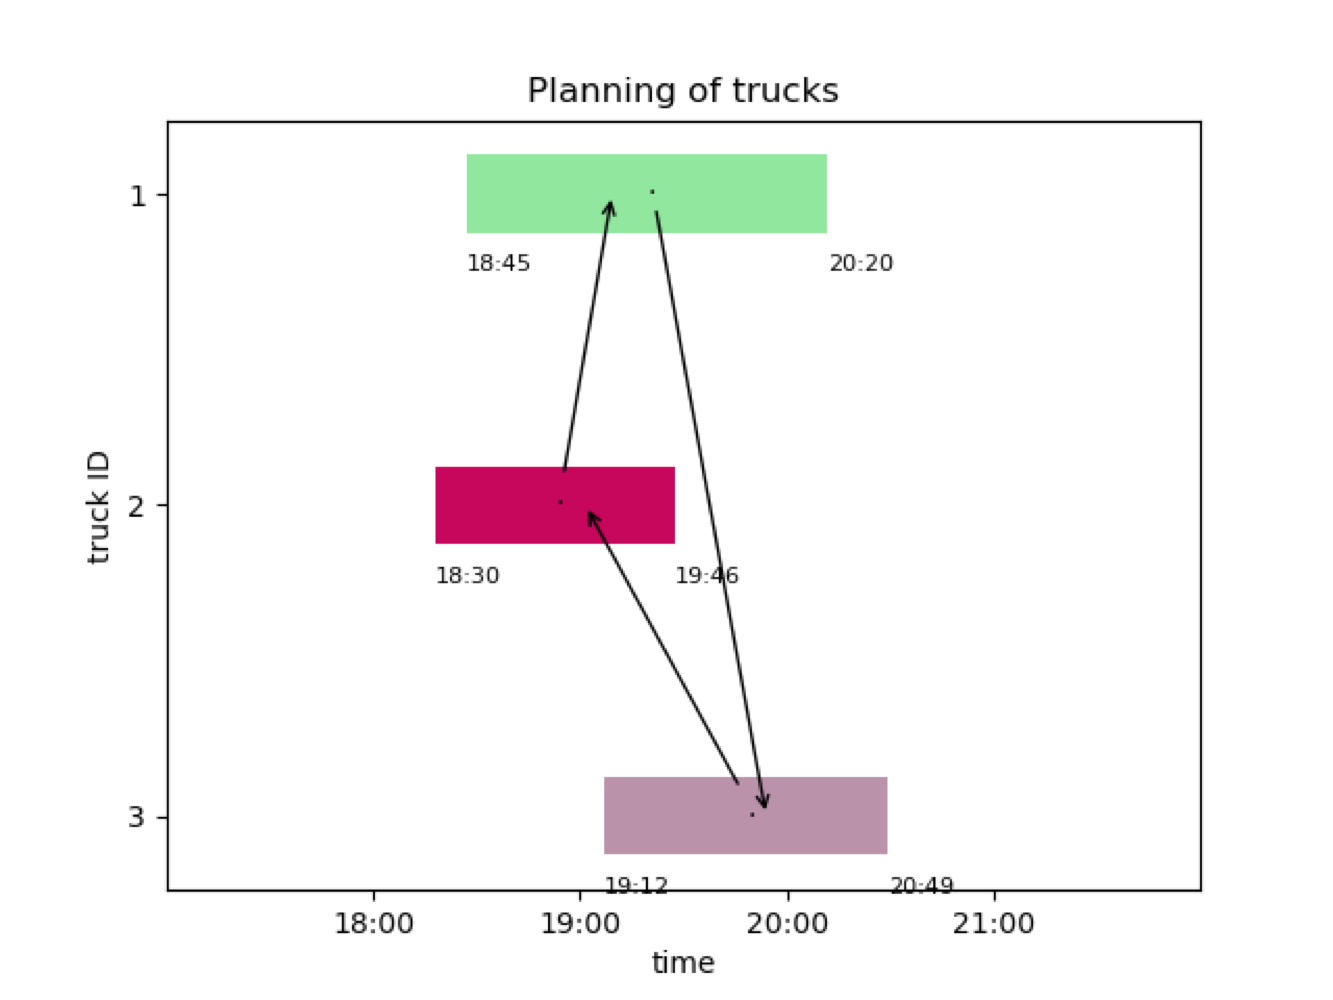
\includegraphics[scale=0.17]{images/exemple1Planning.png}
      \caption{A previsional planning of trucks with arrival/departure times. Arrows indicate a transfert of pallets $f_{ij}$ between trucks $i$ and $j$.}
      \label{fig:second}
    \end{subfigure}
    \caption{Data of the crossdock and the planning of trucks for the illustration example}
    \label{fig:Example1}
    \end{figure}

  
\vspace{-4mm}
\paragraph{Regarding the cross-dock}
\begin{itemize}
    \item It is composed of: 
    
      $M=\{1,2,3\}$, three docks ($m=3$)
      according to the layout illustrated in Figure \ref{fig:layoutexample}.
    
    \item The times of transfer between docks (in minutes, $0\le$ minute $\le59$) are given by:    
    
       $t=\begin{pmatrix} 
        0&1&4 \\ 
        1&0&3 \\  
        4&3&0
        \end{pmatrix}$ 

   \item There is no restriction on the capacity (in number of pallets) in this example:
   
      $C=\infty$    
   
\end{itemize}

 
\paragraph{Regarding the previsional planning of trucks and transfers of pallets}

\begin{itemize}
    \item The scenario is composed of: 
    
     $N=\{1,2,3\}$, three trucks ($n=3$)

    \item The hours of arrival and of departure (in format hour.minute, $0\le$ hour $\le 23 $, $0\le$ minute $\le59$) are known and are, respectively for each trucks: 
    

      $a=(18.45,\ 18.30,\ 19.12)$\\    
     $b=(20.20,\ 19.46,\ 20.49)$   

    \item The transfer of pallets between trucks: 

     $f=\begin{pmatrix} 
    0&0&1 \\ 
    1&0&0 \\  
    0&1&0
   \end{pmatrix}$  states  
   $\begin{cases}
     \mbox{truck 1 delivers 1 pallet to truck 3}\\
     \mbox{truck 2 delivers 1 pallet to truck 1}\\
     \mbox{truck 3 delivers 1 pallet to truck 2}
   \end{cases}$
   
\end{itemize}


\paragraph{Regarding the costs}

\begin{itemize}
    \item The operational costs and the penalty costs (in euros, at the format unit.cents) are respectively:  
    
       $c=\begin{pmatrix} 
              0.0 & 1.0 & 1.0 \\ 
              1.0 & 0.0 & 2.0 \\  
              1.0 & 2.0 & 0.0
            \end{pmatrix}$
%    
      \ and \ $p=\begin{pmatrix} 
              0.0 & 0.0 & 52.0 \\ 
              24.0 & 0.0 & 0.0 \\  
              0.0 & 23.0 & 0.0
            \end{pmatrix}$
         \smallskip 
\end{itemize}
 
 
\paragraph{Regarding the derivated data}
\begin{itemize}
    \item The vector $\hat{x}$ indicates if a pair of trucks has a conflict or not between their times windows; the value \texttt{1} means ``no conflict'' and the value \texttt{0} shows ``a conflict'':  
    
    $\hat{x}=\begin{pmatrix} 
    0&0&0 \\ 
    0&0&0 \\  
    0&0&0
   \end{pmatrix}$  states 
   $\begin{cases}
     \mbox{the time window of truck 1 is in conflict with trucks 2 and 3}\\
     \mbox{the time window of truck 2 is in conflict with trucks 1 and 3}\\
     \mbox{the time window of truck 3 is in conflict with trucks 1 and 2}
   \end{cases}$

   \item The vector $\tau$ collects all the hours of arrival and departure in one sorted vector: 

      $\tau = (18.30,\ 18.45,\ 19.12,\ 19.46,\ 20.20,\ 20.49)$ 

\end{itemize}

  
\vspace{-4mm}
\paragraph{A feasible solution}

\begin{itemize}
    \item The three trucks can be assigned at one of the three docks, as depicted by Figure \ref{fig:Example1Solution}.
   % \vspace{-3mm}
    
        \begin{figure}[h!]
            \begin{minipage}[t]{0.4\textwidth}
                \hspace{10mm}
                    $\begin{cases}
                         \mbox{truck 1 assigned to dock 1}\\
                         \mbox{truck 2 assigned to dock 2} \ \longrightarrow \\
                         \mbox{truck 3 assigned to dock 3}
                    \end{cases} $
             \end{minipage}
             \begin{minipage}{0.7\textwidth}
                 \centering
                 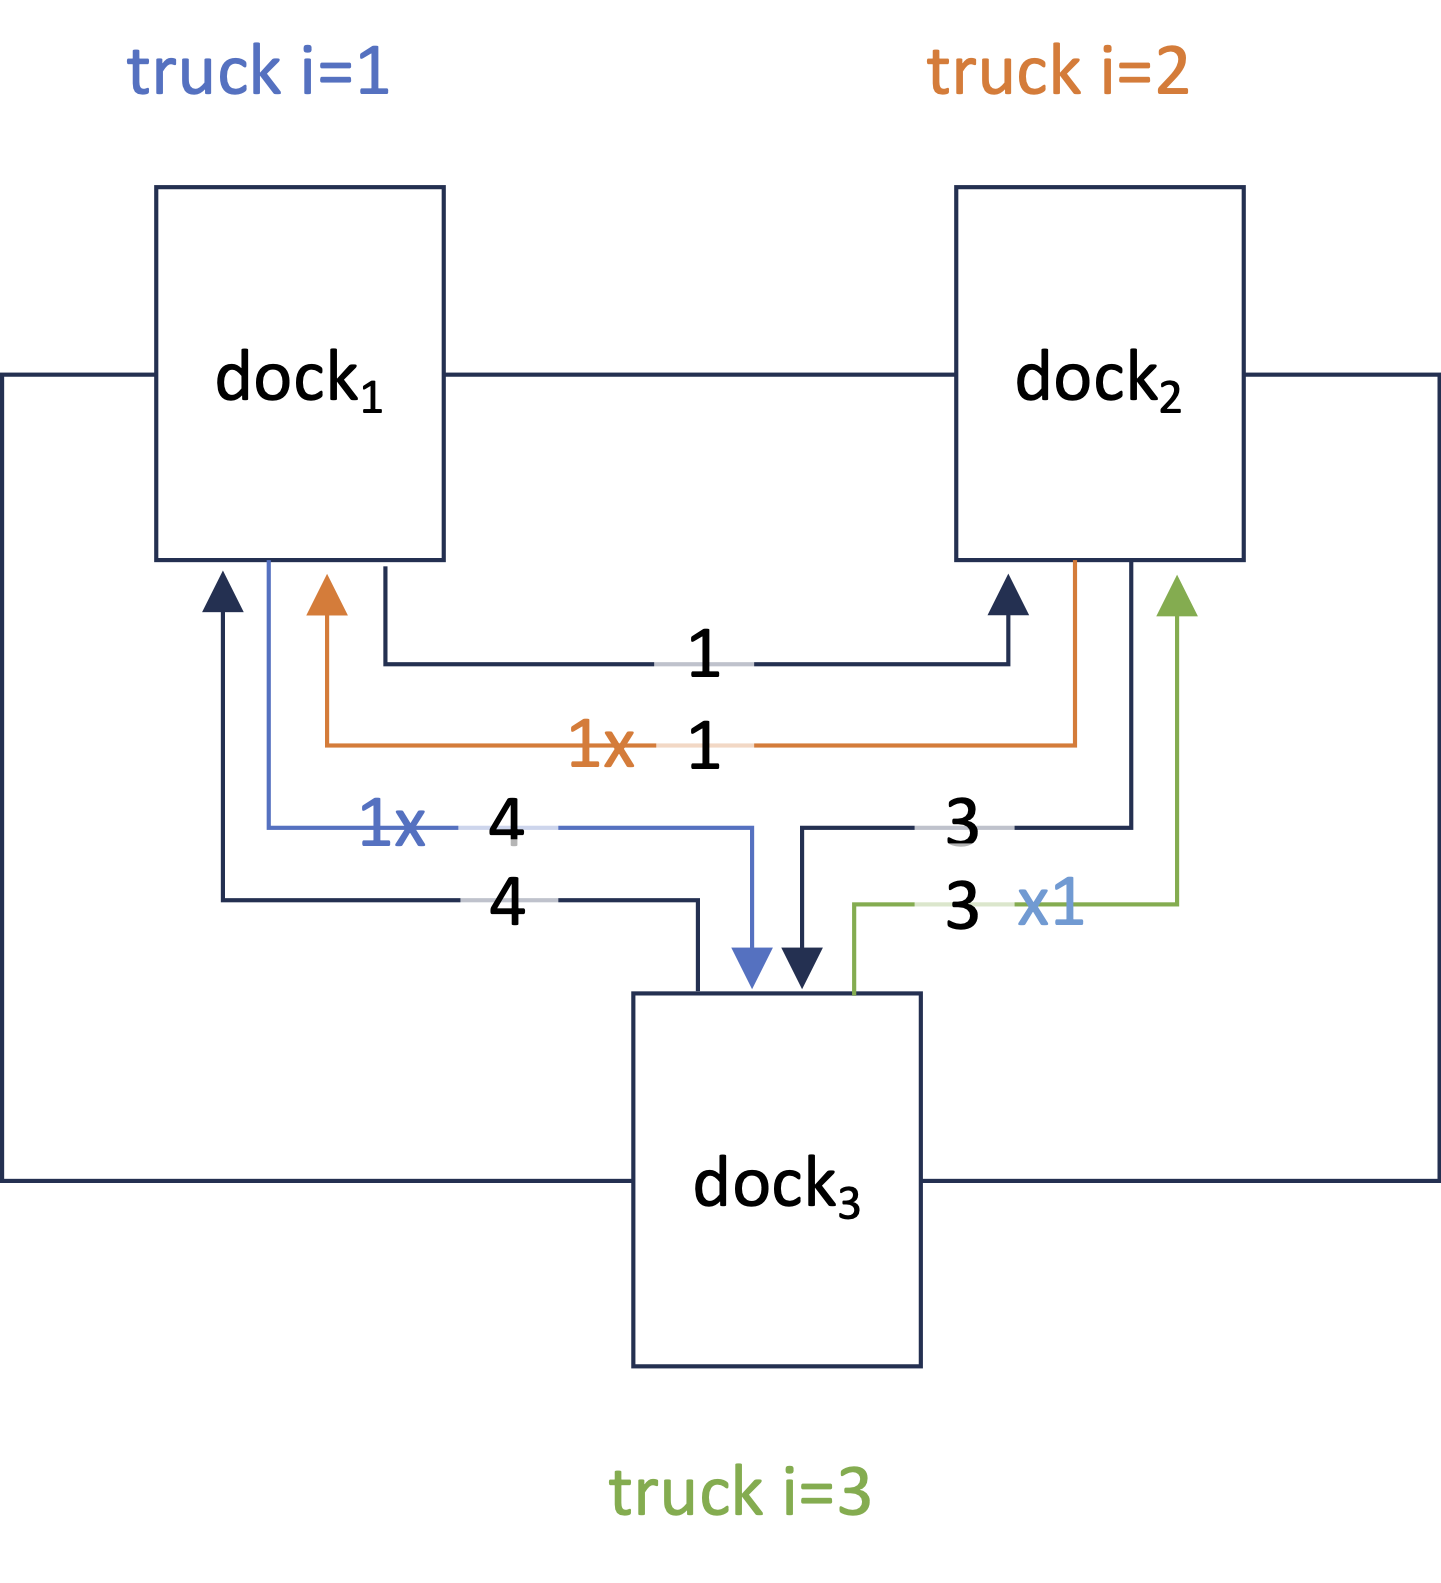
\includegraphics[scale=0.12]{images/exemple1Solution.png} 
             \end{minipage}
             \caption{Assignment of trucks to docks and the corresponding transfers of pallets within the cross dock.}
             \label{fig:Example1Solution}
           \end{figure}  
    
    
    \item There is no conflict between the time windows and enough time to make all pallet transfers:
        \begin{itemize}
        \item trucks 1 and 3 are together for 68 minutes (20h20-19h12) on the crossdock.

        \item trucks 2 and 1 are together for 61 minutes (19h46-18h45) on the crossdock.

        \item trucks 3 and 2 are together for 34 minutes (19h46-19h12) on the crossdock.
        \end{itemize}


    \item The transfer times of pallets between docks (unit of time x number of pallets) thereby are: 
    
        \begin{itemize}
        \item 1 pallet of truck 1 (dock 1) to truck 3 (dock 3): \\
        transfer time of 4 minutes (= 4 minutes  x 1 pallet)

        \item 1 pallet of truck 2 (dock 2) to truck 1 (dock 1): \\
        transfer time of 1 minute (= 1 minute  x 1 pallet)

        \item 1 pallet of truck 3 (dock 3) to truck 2 (dock 2): \\
        transfer time of 3 minutes (= 3 minutes x 1 pallet)
        \end{itemize}

        which make a total of $4 + 1 + 3 = 8$ unit of time (minutes) for all the pallets. All the pallets have been transferred, no penalty appears in this example.

\end{itemize}

%
% =======================================================================
% =======================================================================
%
\section{Formulation M}\label{sec:FormulationM}


The original IP model introduced by \cite{MIAO2009} is stated as follow.
%
Two sets of decision variables are defined:
\medskip

%\begin{itemize}
    %\item [] 
    $y_{ik} \hspace{2mm} = 
      \begin{cases} 
        1  \ \text{if truck $i$ assigned to dock $k$}  \hspace{45mm} (1\le i \le n;\ 1\le k \le m) \\ 
        0  \  \text{otherwise} 
      \end{cases}$ 
\smallskip

    %\item [] 
    $z_{ijkl} = 
    \begin{cases} 
      1 \ \text{if truck $i$ assigned to dock $k$, truck $j$  to dock $l$} \hspace{5mm} (1\le i,j \le n;\ 1\le k,l \le m)\\ 
       0  \ \text{otherwise} 
     \end{cases}$
%\end{itemize}
\bigskip

\noindent
The model is thus formulated as: \\
\begin{equation*}
\begin{array}{ll@{}ll}
\text{min}  & \displaystyle\sum\limits^{m}_{k=1} \sum^{m}_{l=1} \sum^{n}_{i=1} \sum^{n}_{j=1} c_{kl} \, t_{kl} \, z_{ijkl} \ + \ \sum^{n}_{i=1} \sum^{n}_{j=1} p_{ij} \, f_{ij} \left( 1-\sum^{m}_{k=1} \sum^{m}_{l=1} z_{ijkl} \right) & \quad  (1) \vspace{2mm}\\
%
\text{s.t.}   & \displaystyle\sum\limits^{m}_{k=1} y_{ik} \leq 1  \hfill (1\le i \le n) & \quad (2) \vspace{2mm}\\
                    & z_{ijkl} \leq y_{ik}   \hfill  (1\le i,j \le n;\ 1\le k,l \le m) & \quad (3) \vspace{2mm}\\
                    & z_{ijkl} \leq y_{jl}   \hfill  (1\le i,j \le n;\ 1\le k,l \le m) & \quad (4) \vspace{2mm}\\
                    & y_{ik} + y_{jl} - 1 \leq z_{ijkl}   \hfill  (1\le i,j \le n;\ 1\le k,l \le m) & \quad (5) \vspace{2mm}\\
                    & \hat{x}_{ij} + \hat{x}_{ji} \geq z_{ijkk}   \hfill  (1\le i,j \le n, i \neq j;\ 1\le k \le m)  & \quad (6) \vspace{2mm}\\
                    & \displaystyle\sum\limits_{k=1}^{m} \sum_{l=1}^{m} \sum_{i\in\{i:a_{i} \le \tau_r\}} \sum_{j=1}^{n} f_{ij} \, z_{ijkl}- \sum_{k=1}^{m} \sum_{l=1}^{m} \sum_{i=1}^{n} \sum_{j\in\{j:d_{j} \le \tau_r\}} f_{ij} \, z_{ijkl} \le C \hspace{6mm}  \hfill (1\le r \le 2n) & \quad (7) \vspace{2mm}\\ 
                    & f_{ij} \, z_{ijkl} \, (d_{j} - a_{i} - t_{kl}) \ge 0   \hfill  (1\le i,j \le n;\ 1\le k,l \le m) & \quad (8) \vspace{2mm}\\
                    & y_{ik} \in \{0,1\}, \ y_{jl} \in \{0,1\}, \ z_{ijkl} \in \{0,1\}   \hfill  (1\le i,j \le n;\ 1\le k,l \le m) &  \quad (9) \\
\end{array}
\end{equation*}

\medskip
\noindent
where:
\begin{itemize}
    \item [(1)] is the objective function, which is composed by the total operational cost (first term) and the total penalty cost (second term);
    \item [(2)] ensures that each truck cannot be assigned to more than one dock;     
    \item [(3-5)] jointly determine the variable $z$ which represent the logic relationship among $y_{ik}$, $y_{jl}$ and $z_{ijkl}$;
    \item [(6)] assures that one dock cannot be occupied by two trucks simultaneously;
    \item [(7)] is the capacity constraint, i.e. for each time point $\tau_r$, the total number of pallets inside the warehouse cannot exceed the capacity $C$;
    \item [(8)] assures that the transfers of pallets from truck $i$ on dock $k$ to truck $j$ on dock $l$ takes place within the time window given by the arrival time of truck $i$ and the departure time of truck $j$;
    \item [(9)] states the integrality of decision variables. 
\end{itemize}
\medskip
The implementation of this formulation in Julia with JuMP is given in \ref{app:JuMPformulationM} and on a GitHub repository available online at \url{https://github.com/xgandibleux/TDAP}.

%
% =======================================================================
%
\subsection{Discussion}\label{sec:discussionM}
\smallskip

%
% --
%
\subsubsection{The objective function given by expression (1)}

The objective is in minimization and contains two parts: the transfer time of the pallets in the cross-dock and the number of undelivered pallets. Those two parts being non-commensurable, they are converted in monetary unit, considering an operationnal cost $c_{kl}$ associated with the transfer of pallets between the docks $k$ and $l$ and a penalty cost $p_{ij}$ associated with a transfer of the truck $i$ to the truck $j$. The two parts can therefore be aggregated into the single synthesis function described by expression (1).

These costs are an artifact that makes the two parts commensurable and play a major role in the aggregation of the two parts. Also, only a single solution may be obtained at the end of the resolution as output of this single objective problem. 
%
However, the two parts are by nature conflictual. Indeed, to minimize transfer times, just don't transfer a pallet, which goes against minimizing the number of undelivered pallets. 
%
Section \ref{sec:Formulation2R} gives the formulation 2R of the TDAP from the perspective of multi-objective optimization. The optimal solutions in the sense of multiple objective optimization (named the efficient solutions and represent compromises regarding the two objectives) are discussed in Section \ref{sec:NumericalExperiments}.

%
% --
%
\subsubsection{The notion of capacity in expression (7)}

The formulation does not help to put in touch the $C$ value with the concrete resource limitations in the cross-dock. Is this value based on a limited number of forklifts, on a congestion related to pallet traffic, on a limitation of pallet handling spaces near the docks, or on an another resource? 

The granularity of the model does not allow us to respond, especially since the time window during which a truck is docked covers three times: unloading, loading and waiting time. No information allows to identify precisely the time  when the pallets are handled within this time window, and therefore to measure accurately the required resources for handling the pallets.

%
% --
%
\subsubsection{The multiplication factor $f_{ij}$ in expression (8)}

The expression (8) raises questions.
%
Indeed, $f_{ij}$ is the expected number of pallets to be transferred between the trucks $i$ and $j$ , with $a_i$ being Truck $i$'s arrival time, $d_j$ Truck $j$'s departure time, and $t_{kl}$ a global time to carry these pallets between the docks $k$ and $l$. 
%
The aim of this constraint is to force the variable $z_{ijkl}$ to zero when the conditions are not gathered to perform this transfer, and (8) is valid in this sense.

%
While the interpretation of the term $f_{ij} \times t_{kl}$ is understandable (although according to the authors, the valuation of $t_{kl}$ includes the number of pallets, and therefore, this product does not represent the time proportional to the number of pallets contrary to what it suggests), this is not the case for $f_{ij} \times d_j$ and $f_{ij} \times a_i$. 
What is the meaning of multiplying a time marker related a truck movement with the number of pallets? In the model 2R described in Section \ref{sec:Formulation2R}, this constraint is modified to clarify this issue. 


%
% =======================================================================
% =======================================================================
%
\section{Literature criticisms about M formulation}
%\subsubsection{Issues and limitations highlighted in }

According to \citet{Gelareh2015,Gelareh2021}, the M formulation has several limitations and issues.
%
They are discussed in the technical report \cite{Gelareh2015} available online and in the paper \cite{Gelareh2021}. The mains criticisms and dedicated corrections are reported hereafter.

%
% =======================================================================
%
\subsection{Mains criticisms and given corrections}

%
% --
%
\subsubsection{No temporary storage}\label{sec:temporary storage}
If there are transfers from a truck $i$ to another truck $j$ and from $j$ to $i$, and one of them is not feasible, then the constraint $(5)$ invalidates both of them.
%
As a consequence of this, if given their time windows truck $i$ can transfer pallets to the truck $j$, these transfers are also not achieved.
%
This is due to the fact that, to make a pallet transfer feasible between two trucks in formulation M, they must be docked with a common period of time which must be long enough for completing the transfer.

The authors consider this restriction as a limitation. 
For them, pallets from truck $i$ may be temporary stored into the cross-dock in waiting for the arrival of truck $j$ to pick them up, even if $i$ has already left the cross-dock.
%
The authors introduce a notion of ``buffer'' and they come with modifications on the M formulation so as to allow temporary storage of pallets.


%
% --
%
\subsubsection{Bi-directional transfer}
There is a link between $z_{ijkl}$ and $z_{jilk}$. Indeed, there is a bi-directional transfer between the two trucks $i$ and $j$ when they share a common time window while they are docked, i.e. $z_{ijkl} = z_{jilk}$ holds.
%
{{This means that there is an equivalent solution where 
truck $j$ is assigned to dock $l$ and truck $i$ is assigned to dock $k$, in which $z_{ijkl} = z_{jilk}$ also holds.}} 

To address this issue, the definition of these variables has been revised so that $z_{ijkl}=1$ if and only if there is an actual transfer from $i$ to $j$. 
Furthermore, using a temporary storage makes the constraint $(6)$ obsolete. It comes from the fact that (i) contrary to the model M, a same dock $k$ can now be used to do a transfer from truck $i$ to truck $j$ and (ii) $j$ does not need to share a common docking time with $i$ and can arrive at any time after the departure of $i$.
Thus, the constraint (6) is revised so that a transfer is able to use the buffer to make deliveries on a same dock $k$. 

%
% --
%
\subsubsection{Extra transportation costs}\label{sec:extratransportationcosts}

The authors have also pointed out others unintended consequences over the optimal solutions induced by the M formulation.

We saw that a bidirectional transfer raises a problem if, for $i,j$ such that $i \neq j$, $f_{ij}=0$ and $f_{ji} > 0$ (case where truck $j$ leaves before truck $i$ arrives). In such occurences, $j$ will drop its cargo in cross-dock buffer for $i$ can pick it up later. 
%
However, since $f_{ij}=0$, constraint (8) is satisfied without any restriction on $z_{ijkl}$, if for some $k,l$ $z_{jilk}=1$, by symmetry, $z_{ijkl}=1$ even though there is no transfer. Because of the first part of the objective function, i.e. $\sum^{m}_{l=1} \sum^{m}_{k=1}\sum^{n}_{i=1} \sum^{n}_{j=1} c_{kl} \, t_{kl} \, z_{ijkl}$, an extra cost is paid for a transfer that does not exist. Consequently, optimal values are inaccurate in this case. 
 
To further correct the model, constraint (5) is removed and replaced by new constraints that allow for non-overlaping time windows in the trucks' docking time. Then, together with constraint (6), a transfert between two distinct trucks on a same dock can be performed using the temporary storage.
%
Also, the constraint $(8)$  has been rewritten so that $z_{ijkl}=0$ when $f_{ij}=0$ and when the time window is too short to make a delivery. 

All these modifications led to a revised formulation proposed by the authors and discussed in Section \ref{sec:FormulationG}.


% ---
\subsection{Discussion}

%
% --
%
\subsubsection{Concerning the temporary storage}
 When assuming that a truck $i$ can unload and store its pallets in the crossdock while waiting the arrival of the truck $j$ to pick them up later, the authors assume the existence of a buffer area to temporarily store the pallets. However, this assumption is related to the operational situation to  consider.
    %
    Indeed, a crossdock may not have such buffer zones to store cargo, or cargo may not be stored, even for a short period of time, e.g. when the cargo are subject to cold chain constraint.

This option is not considered in \citep{MIAO2009}, and it changes the nature of the problem considered. Thus it cannot be viewed as a weakness of the formulation M. 
In other words,  formulations M and G  consider two different variants of the TDAP.
 

%
% --
%
\subsubsection{Inaccuracies in documents}
Although the documents \citet{Gelareh2015,Gelareh2021} propose valid technical solutions to limitations and issues raised  in  formulation M, unfortunately these two documents contain themself inaccuracies such as several inconsistent points and typos.

 First, the authors use in these documents an example to demonstrate that the M formulation does not compute all the feasible solutions. The example is built so that M find no solution and forbid all transfers while the G formulation should find solution. 

 \begin{itemize}
     \item With  the formulation M, they report a value of 16 for the objective function, and none of the variable is activated, which is different from the sum of penalties when no transfer is fulfilled, namely 22.

Indeed, given the definition of the objective function (1) in formulation M, when  all variables $z_{ijkl}=0$  with 11 transferts to consider, a penalty value of 1 for each unfullfiled transfert, and 2 pallets per transfert, the penalty term gives:

$\sum^{n}_{i=1} \sum^{n}_{j=1} p_{ij} \, f_{ij} \left( 1-\sum^{m}_{k=1} \sum^{m}_{l=1} z_{ijkl} \right) = 2 \times 1 \times 11 = 22$

\item With  the formulation G, the value of 11 is reported, with 5 variable activated.
However, with $c_{kl} = t_{kl} = 1 $ the terms corresponding to the transfert and the penalty take respectively the values 5 and 6: \\
$1\times1\times5 \ \ + \ \ 1\times2\times6 = 17$
\vspace{0mm}

Here again, the value reported is different.
With the information provided in the documents, to the best of our capabilities, we were not able to understand the origin of these differences. 
 \end{itemize}


Second, the formulation G published by the authors does not allow to reproduce the results reported in the papers. 
%
Indeed, the description of the formulation given in both documents is the same but it contains several errors and missing information to implement it properly, see Section \ref{sec:FormulationG} for details. Some corrections of these deficiencies can be inferred with certainty, others are subject to interpretation.
%
After correcting the errors identified, the fixed formulation was implemented in JuMP (see \ref{app:JuMPformulationG}) and solved to optimality using GUROBI as MIP solver and using the datasets (see Section \ref{sec:fullmesh}) provided online by these authors.
Unfortunately none of the numerical experiments has led us to the optimal value announced in papers for the given instances.
%  All solutions we obtained are dominated on all instances (see table \ref{subtab:G_results} and \ref{tab:table_R_results}) and the observed difference in the objective value can be up to twice as large.
 %
 Because the authors do not mention any open access to their codes,  it is not possible to determine the origin of divergence between both implementations. 
 %
This fixed formulation will be the basis for the formulation 2R proposed and presented in Section \ref{sec:Formulation2R}.   


%
% =======================================================================
% =======================================================================
%
\section{Formulation G}\label{sec:FormulationG}

The IP model corresponding to the formulation G uses the same definition of the decision variables  of  the formulation M.
%
The formulation is reproduced exactly as  described in \citep{Gelareh2015,GELAREH2016,Gelareh2021} in  \ref{app:formulationsGoriginale}, with errors and missing information.
%
%uses ).
%
Indeed, a number of inaccuracies and incompleteness were identified in formulation G, making this formulation non-operational.
%
They are listed and a proposed correction is reported in \ref{app:CorrectionsG}.

Taken individually each of these points can be corrected quite easily once identified. 
%
However, some are not immediately identifiable, 
%as in the case of the point relating to constraint (5), 
which could only be found after a meticulous analysis of the flat formulation, which necessitated testing instances by hand.
%
In addition, when the indices are missing or in excess, or when their values are not stated, this leads to confusion and ambiguity of expression, exposing us to the possibility of deviating from the authors' original intentions.

We have therefore made the corrections, which have enabled us to obtain a formulation that provides consistent solutions. 
Unfortunately, we were unable to reproduce the results announced by the authors.
%
The implementation  in Julia with JuMP after having fixed issues of this formulation is given in \ref{app:JuMPformulationG} and on a GitHub repository available online at \url{https://github.com/xgandibleux/TDAP}.    

%
% =======================================================================
%
\subsection{Discussion}\label{sec:discussionG}
\smallskip

%
% --
%
\subsubsection{Storage capacity}

The question of the overall capacity constraint expressed by 
%
 $$\sum\limits_{k=1}^{m} \sum_{l=1}^{m} \sum_{i\in\{i:a_{i} \le \tau_r\}} \sum_{j=1}^{n} f_{ij} \, z_{ijkl} \ \color{black}{-}\color{black} \ \sum_{k=1}^{m} \sum_{l=1}^{m} \color{black}\sum_{i=1}^{n}\color{black} \sum_{j\in\{j:d_{j} \le \tau_r\}} f_{ij} \, z_{ijkl} \le  C \hspace{1mm}$$
 \hfill $ \forall r \in \{1,2,...,2n\} \quad (7)$
 
\bigskip
\noindent
which does not discriminate the allowed storage in the formulation G.
%  
This point has already been discussed in the analysis of formulation M.
This concern is more relevant in formulation G, in particular when the time windows of trucks $i$ and $j$ have no intersection. In this situation, pallets from $i$ must therefore be stored while awaiting the arrival of $j$.
    %
    In order to grasp this aspect more realistically, a perspective could be to consider capacity constraints attached to platforms, as for the Cross-Docking Assignment Problem (CDAP) \citep{Zhu2009} .      

%
% --
%
\subsubsection{The case of pallets not transfered.}\label{sec:palletnotTransferred}

With formulations M and G, and numerical instances used in papers \cite{GELAREH2016,MIAO2009},  in an optimal solution, when a pallet cannot be transferred, it remains in the truck. However a capacity problem may occurs here. Indeed, if this truck is initially planned to leave the crossdock fully loaded with pallets issued from other trucks, an infeasible situation occurs (truck loaded over its capacity) but is not managed by the model. 
%
A way to deal with these cases is to consider planning with incoming and outcoming trucks, where incoming trucks do not receive pallets. Thus, a pallet not transferred is returned to the furnisher. The new numerical instances that we produced (see Subsection \ref{sec:bipartite}) are inspired from existing instances for the CDAP, and then are compliant with this policy.
   


%
% =======================================================================
% =======================================================================
%
\section{Formulation 2R}\label{sec:Formulation2R}

The formulation 2R (R stand for Revised, 2 for two objectives) is now presented.
%
Founded on the formulation G where all the corrections that we proposed are integrated, this formulation is basically a rigorous description of the formulation G  revisited. Indeed, it comes with a redefinition of one constraint (referred by expression (8) hereafter), plus several changes underlined along the discussions in the preceding sections.

The decision variables are identical to the formulations M and G.
%
The expression (1) giving the objective function in of M and G is spitted in two parts, giving the two objectives functions without the artifacts $c_{kl}$ and $p_{ij}$:  (1.1) minimize the transfer time of the pallets in the cross-dock and (1.2) minimize the number of undelivered pallets. 
%
The IP model is formulated as follow: \\
\begin{equation*}
    \begin{array}{ll@{}ll}
    \text{min}  & \displaystyle\sum\limits^{m}_{k=1} \sum^{m}_{l=1} \sum^{n}_{i=1} \sum^{n}_{j=1} t_{kl} \, z_{ijkl} \  &  \hspace{4mm} (1.1) \vspace{2mm}\\
    \text{min} & \displaystyle\sum^{n}_{i=1} \sum^{n}_{j=1} f_{ij} \left( 1-\sum^{m}_{k=1} \sum^{m}_{l=1} z_{ijkl} \right)   &  \hspace{4mm} (1.2) \vspace{2mm}\\
    %
    \text{s.t.}     & \displaystyle\sum\limits^{m}_{k=1} y_{ik} \leq 1   \hfill   \forall i \in N & \quad (2)\vspace{1mm}\\
                    & z_{ijkl} \leq y_{ik}   \hfill   \forall i\in N, \ j \in N, \ k \in M, \ l \in M & \quad (3)\vspace{2mm}\\
                    & z_{ijkl} \leq y_{jl}   \hfill   \forall i\in N, \ j \in N, \ k \in M, \ l \in M & \quad (4) \vspace{2mm}\\
                    & y_{ik} + y_{jk} \leq 1 + \hat{x}_{ij} + \hat{x}_{ji}   \hfill   \forall i\in N, \ j \in N, \ k \in M,  \ i \neq j & \quad (5)  \vspace{2mm}\\
                    %&   \hfill   i \neq j &  \vspace{2mm}\\
                    & z_{ijkk} \leq \hat{x}_{ij}   \hfill   \forall i\in N, \ j \in N, \ k \in M, \  i \neq j &  \quad (6)  \vspace{1.5mm}\\
                    %&   \hfill   i \neq j &  \vspace{1mm}\\
                    & \displaystyle\sum\limits_{k=1}^{m} \sum_{l=1}^{m} \sum_{i\in\{i:a_{i} \le \tau_r\}} \sum_{j=1}^{n} f_{ij} \, z_{ijkl} \ - \ \sum_{k=1}^{m} \sum_{l=1}^{m} \sum_{i=1}^{n} \sum_{j\in\{j:d_{j} \le \tau_r\}} f_{ij} \, z_{ijkl} \le  C \hspace{0.5cm} & \quad  (7)  \vspace{1mm}\\ 
                    &  \hfill  \forall r \in \{1,2,...,2n\}&  \vspace{3mm}\\ 
                    & z_{ijkl} = 0   \hfill  \forall i\in N, \ j \in N, \ k \in M, \ l \in M, \  i \neq j, & \quad (8)\\
                    %&   \hfill  i \neq j, \\
                    &   \hfill   (d_j - a_i - f_{ij} \, t_{kl} \leq 0) &  \vspace{2mm}\\
                    & y_{ik} \in \{0,1\}   \hfill  \forall i\in N, \ k \in M & \quad  (9) \vspace{2mm}\\
                    & z_{ijkl} \in \{0,1\}   \hfill   \forall i\in N, \ j \in N, \ k \in M, \ l \in M & \quad  (10) 
                    \vspace{2mm}\\
    \end{array}
\end{equation*}
%\smallskip

Compared to the formulation G corrected, the constraint (8) is adapted in the formulation 2R.
%
Indeed, in the formulation G, the parameter $t_{kl}$ is considered as a global value. This value is initially established independently of the quantity of pallets really convoyed from $k$ to $l$.
%
In formulation 2R, $t_{kl}$ is the unitary time required by a forklift to do a round trip when it moves a pallet from $k$ to $l$.
With this adaptation, the formulation takes into consideration the real quantity $f_{ij}$ of pallets convoyed into account in the computation of the time required for transferring all the pallets from $k$ to $l$.

The implementation of this formulation in Julia with JuMP is given in \ref{app:JuMPformulation2R} and on a GitHub repository available online at \url{https://github.com/xgandibleux/TDAP}.
\medskip

%
%\begin{equation*} \label{}
%    \begin{array}{ll@{}ll}
%    \text{min}  & \displaystyle\sum\limits^{m}_{k=1} \sum^{m}_{l=1} \sum^{n}_{i=1} \sum^{n}_{j=1} t_{kl} \, z_{ijkl} \ & \hspace{20mm} & (1.1) \vspace{2mm}\\
%    \text{min} & \displaystyle\sum^{n}_{i=1} \sum^{n}_{j=1} f_{ij} \left( 1-\sum^{m}_{k=1} \sum^{m}_{l=1} z_{ijkl} \right)  & & (1.2) \vspace{6mm}\\
%    %
%    \text{s.t.}     &  \mbox{constraints } (2)-(10) \mbox{ of formulation R } \vspace{2mm}\\
%    \end{array}
%\end{equation*}


\subsection{Comments on the formulation 2R}

\label{sec:2.5.2}

A crucial aspect to grasp for an overall understanding of the formulation 2R is the role that represents the matrices $t_{kl}$ and $f_{ij}$. By making these two unitary values, we can represent the transfers as a ``flow" of pallets ($t_{kl} \times f_{ij}$) which was not possible with formulations M and G, $t_{kl} $ and $f_{ij}$ being independent values in those formulations. Another aspect of these two matrices is that their unit is not always specified in papers on M and G. For the formulation 2R and the associated instances, we consider $t_{kl}$ as fractional hours and $f_{ij}$ as a number of pallets.

%Concerning  the objective function In the formulation 2R, the interpretation of $t_{kl}$ changes and no longer represents the total operational time required for a transfer from dock $k$ to dock $l$. This change means that the operational cost of a transfer corresponding to $t_{kl} \times c_{kl}$ in formulations M and G is now $t_{kl} \times c_{kl} \times f_{ij} $ in the formulation R. The operational cost being used in the objective function, we can substitute the current expression with the most faithful one. Finally, this approach does not hinder any transfer or exchange, but if one wants to represent situations more faithfully to reality, this adaptation is in our opinion essential.

%It should be noted that for the same instance file, the G and R formulation, even if similar, will not give the same results because they do not interpret the data in the same way. For example, suppose a transfer from a truck $i$ at dock $k$ to a truck $j$ at dock $l$ such that $t_{kl} = 1$ and $f_{ij} = 5$ with $t$ in hour and $f$ in number of pallets. For the formulation G, this situation represents a transfer of 5 pallets taking a total of 1 hour, while the formulation R interprets this situation as the transfer of 5 pallets each lasting 1 hour, i.e. 5 hours in total. This must be taken into account in order to be able to compare the results in the annexe.



 
\newpage    
%
% =======================================================================
% =======================================================================
%
\section{Numerical experiments} 
\label{sec:NumericalExperiments}

%
% =======================================================================
%
\subsection{Numerical Instances}

%
% ===
%
\subsubsection{Instances ``full mesh''}\label{sec:fullmesh}

The experiments reported by \citet{MIAO2009} have been conducted with a collection of instances that represent a crossdock with a I-shape, where dock gates are symmetrically located on each sides. Datasets have been randomly generated  (i) with different values of parameters $n$ and $m$, and (ii) with the following characteristics:
\begin{itemize}
    \item the time window of a truck on a dock is randomly comprised between 45 minutes at minimum and  74 minutes at maximum;
    \item the  value $f_{ij}$ giving the number of pallets to be shipped is randomly chosen between 6 and 60. %, but only if the receiving truck leaves after the arrival of the giving truck. 
    \item the duration of the transfert $t_{kl}$ is based on the Manhattan distance between two docks gates. The authors specifies that a ``proportional conversion" is necessary to define $t_{kl}$ correctly but without more detail. 
\end{itemize}
%

Note that, any truck can carry out a pallet transfer to all the other trucks (see Figure~ \ref{fig:fluxfullmesh}). It is in this sense that we named them "full-mesh". 
\vspace{-5mm}

\noindent 
\begin{figure}[h!]
\begin{minipage}{0.5\textwidth}
\centering
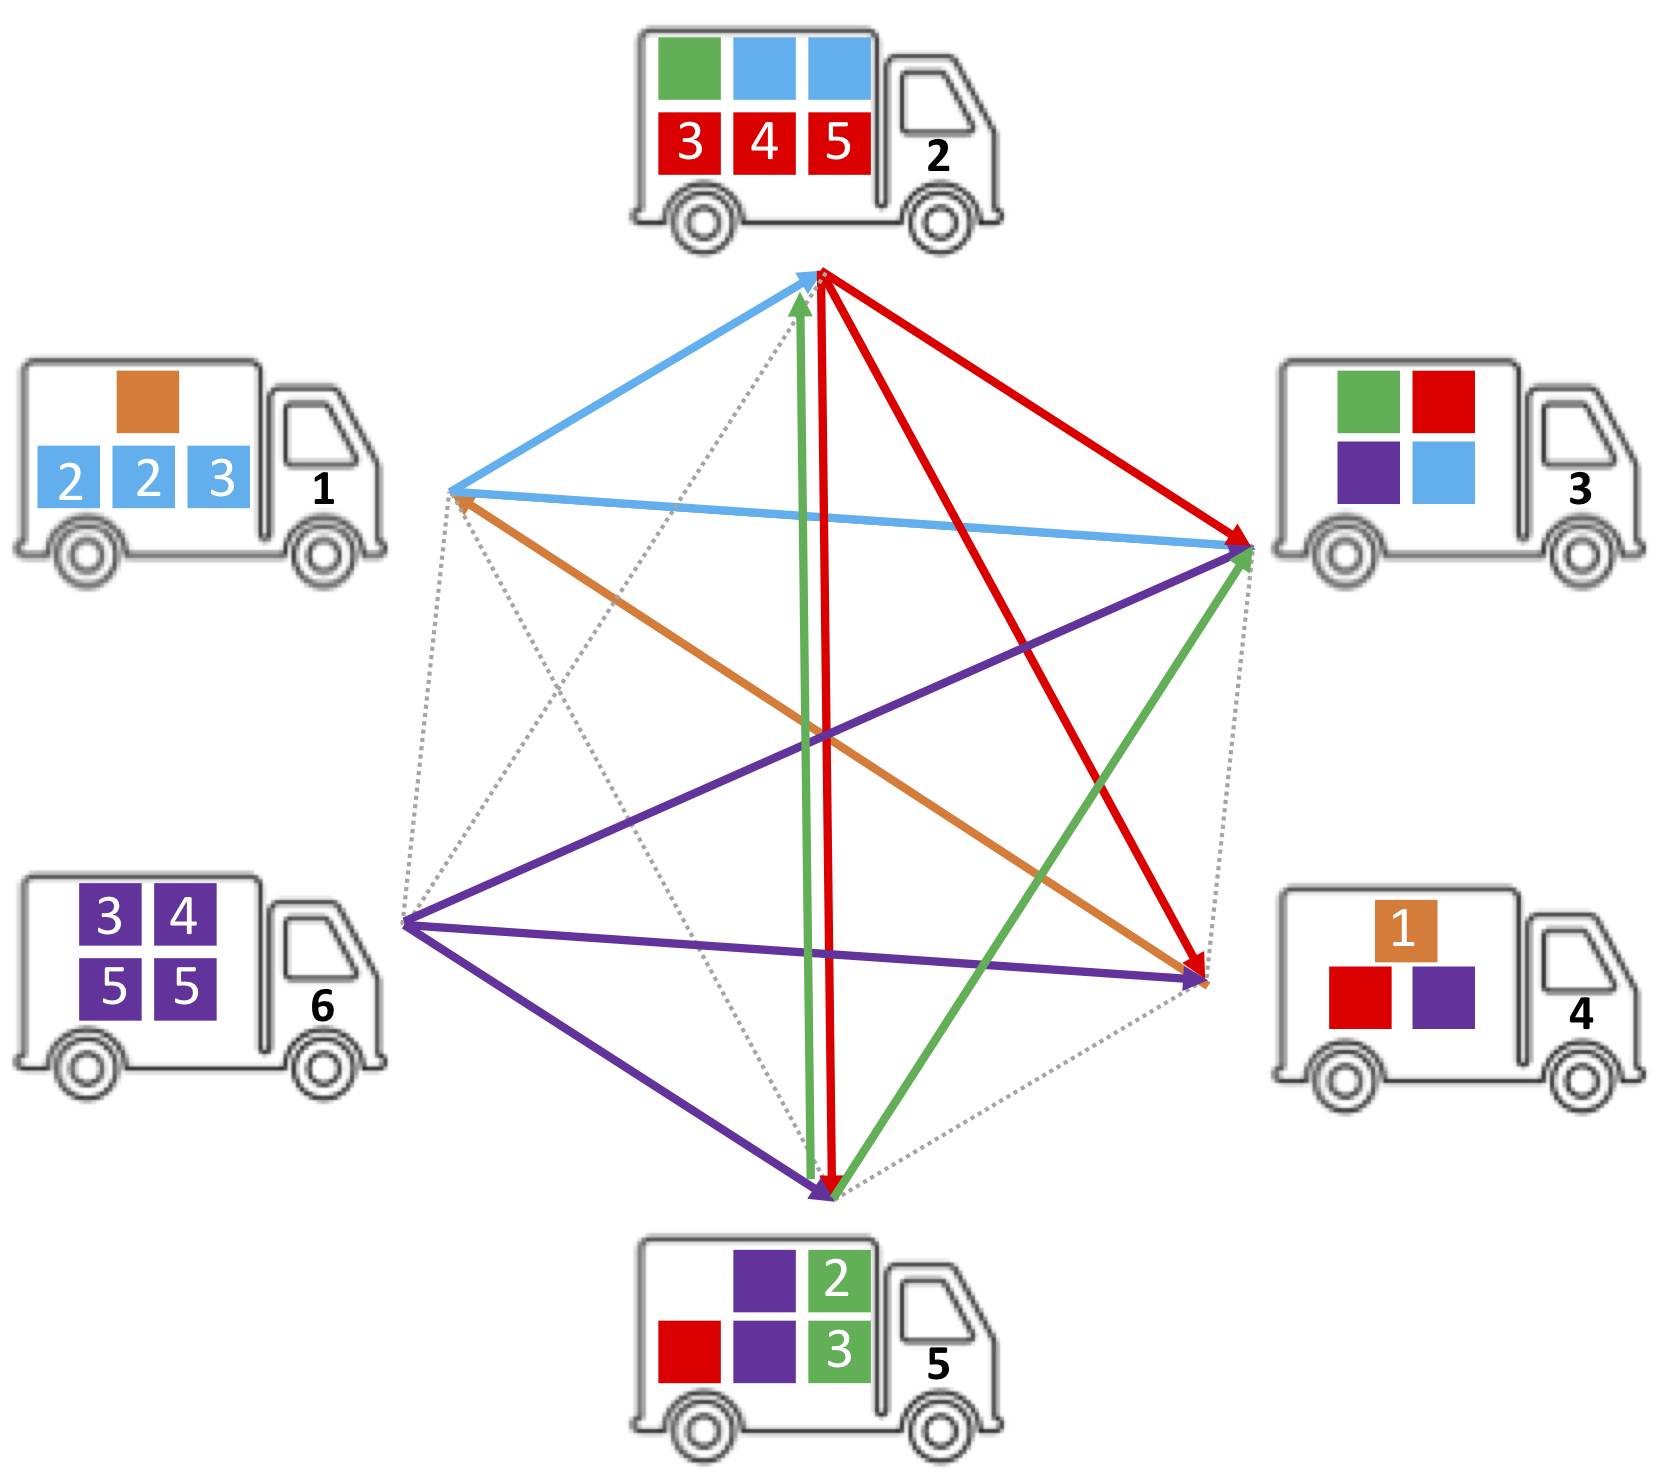
\includegraphics[scale=0.36]{images/fullmesh.png}
\end{minipage}
\begin{minipage}{0.5\textwidth}
\caption{Example of a full-mesh transfer of pallets. Trucks arrives with pallets from furnishers, and leave with pallets to customers. For example, truck numbered 2 arrives with three (red) pallets destined to trucks 3/4/5, and leaves with pallets provided by truck 1 (blue) and truck 5 (green).}
\label{fig:fluxfullmesh}
\end{minipage}
\end{figure}

On base of their size $n \times m$, authors distinguish  three categories of instances,  
%
(1) the \textit{small size instances} ($10 \times 3$ to $18 \times 6$),
(2) the \textit{medium size instances} ($20 \times 6$ to $40  \times 8$), and
(3) the \textit{large size instances} ($50 \times 10$ to $80 \times 12$).
%
Nevertheless, datafiles are not provided by the authors. 


For the paper \citep{Gelareh2015}, authors have generated instances following generation procedure described below.
For the $t_{kl}$, no proportional conversion is considered, only the Manhattan distance is kept.
The datafiles generated are available online\footnote{\url{https://www.lgi2a.univ-artois.fr/~gelareh/downloads/cross_dock/data.rar}} but raise questions about at least 2 aspects.

First, this way of defining transfers from truck $k$ to truck $l$ without ``proportional conversion" implies that there is no link between the duration of a pallet transfer $t_{kl}$ and the quantity of pallet in this transfer $f_{ij}$. These choices can lead to a long transfer time for a small number of pallets to be transferred, which is not in line with a real situation.
%
Second,  the units associated to values such as $t_{kl}$ are not stated.
The units applied to the data is a potential source of inconsistencies that can lead to misuse of the data.  
%
This led us to develop a new set of instances following the generation procedure presented in the next section.

% the duration of some dock-to-dock transfers may end up disproportionated. 
% Indeed, the time required for a transfer in the files is between 0 and $m \in \{3,\ldots,8\}$, the number of docks (in time units). 
% Thus, if they are measured in hours, some transfers take up to 8 hours (the maximum value of $m$) to be completed, which is not realistic. This rules out some possibilities for dock-to-dock transfers, and this makes us question the validity of these instances. 

%
% ===
%
\subsubsection{Instances ``bi-partite''}\label{sec:bipartite}

Based on  data collected and reported in \ref{app:ConsiderationsInstancesBipartite}, 
new  instances aiming to be realistic are proposed for the TDAP.
 

Main differences with instances presented in Section \ref{sec:fullmesh} concerns the trucks.
%
First, a distinction is made between 
``incoming trucks'', those who carry pallets issued from furnishers (factories, other warehouses, etc.), and 
``outcoming trucks'', those who carry pallets to customers (shops, other warehouses, etc.).
%
Next, the fleet of trucks is heterogeneous in the sense of the capacity of incoming trucks is larger than the outcoming ones. 
%
Finally, incoming trucks do not receive pallets from any other trucks. Only outcoming trucks receive pallets. Thus the transfer of pallets can be seen following a bi-partite graph (see Figure \ref{fig:fluxbiparti}), giving the name of this new collection. 


\noindent 
\begin{figure}[h!]
\begin{minipage}{0.5\textwidth}
\centering
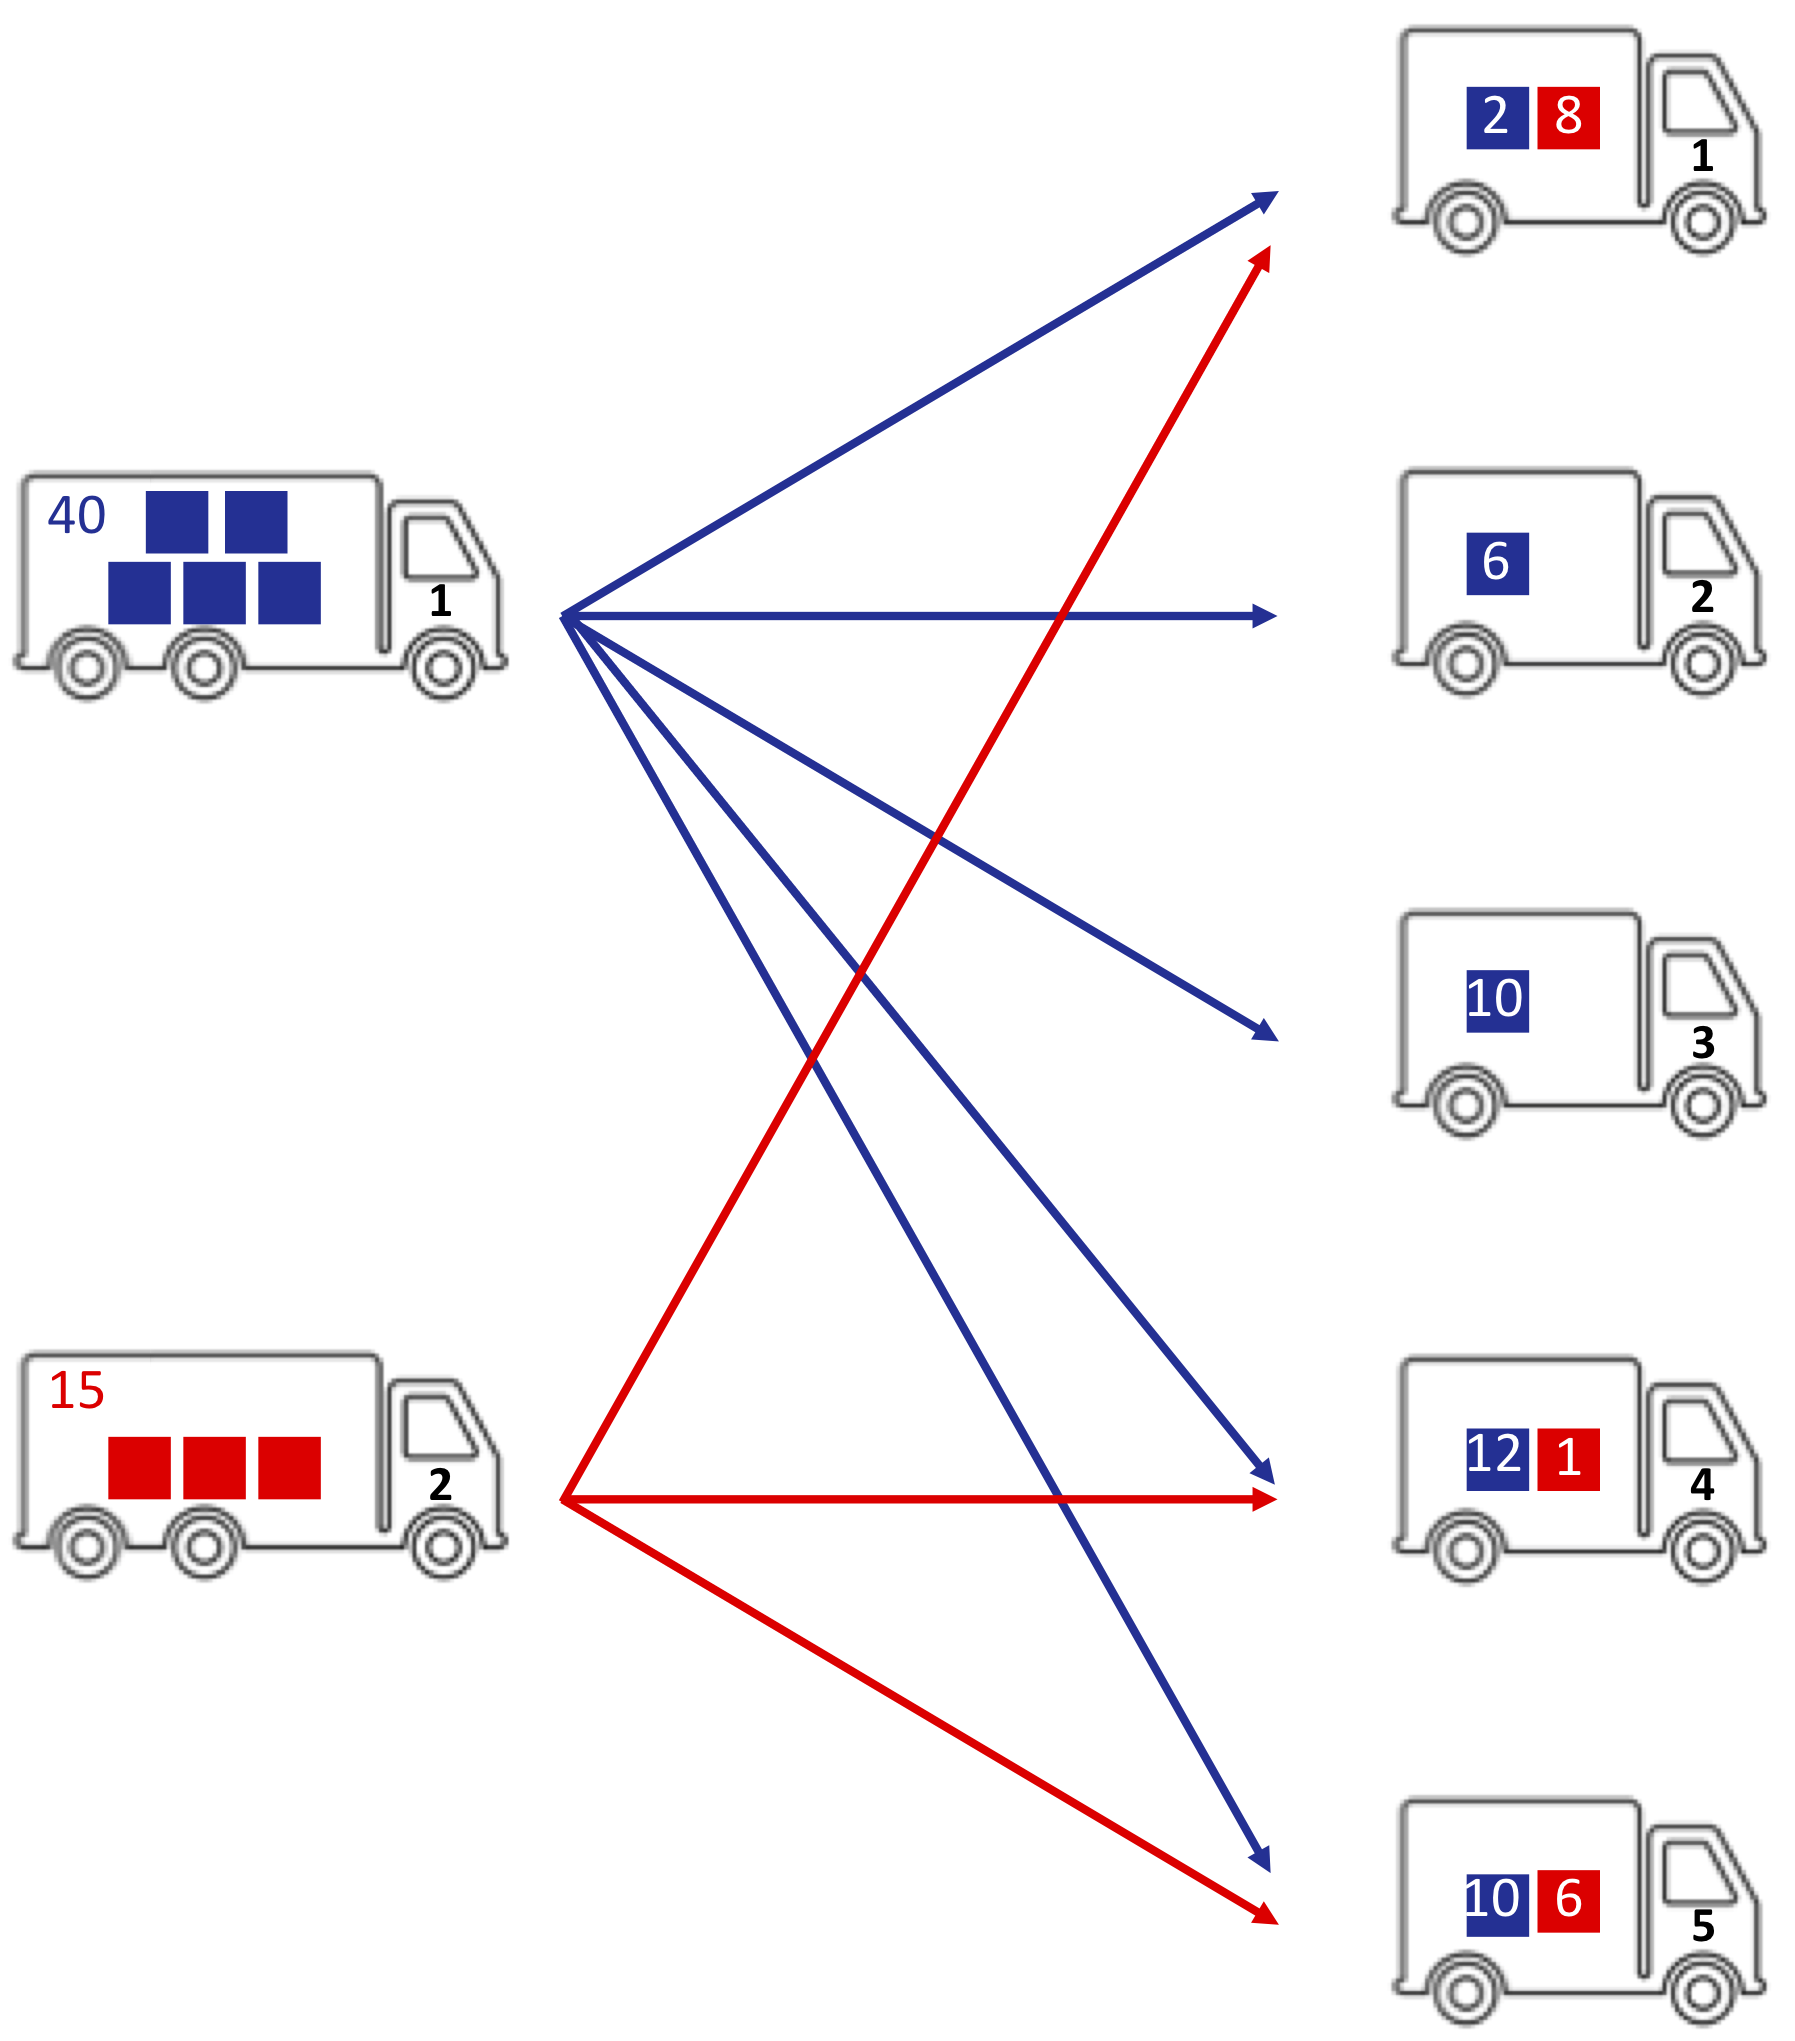
\includegraphics[scale=0.36]{images/fluxbiparti.png}
\end{minipage}
\begin{minipage}{0.5\textwidth}
\caption{Example of a bipartite transfer of pallets. Incoming (and biggest) trucks (on the left) carry pallets from furnishers, outcoming (and smallest) trucks (on the right) carry pallets to customers.}
\label{fig:fluxbiparti}
\end{minipage}
\end{figure}


The instances have been generated according this set of rules: 
%
\begin{itemize}
    \item A crossdock has a layout of ``I'' and presents $m$ docks, with  $4\le m \le 14$.

    \item The distance $dist(k,l)$ between two docks $k$ and $l$ is based on the Manhattan distance. Measures are deduced from the physical configuration of the warehouse.
    
    \item The crossdock has no fix equipment inside. It is viewed as an empty building where the pallets are transfered by forklifts.
    
        \item The transfer time between two docks $k$ and $l$ is computed with the formula $dist(k,l) \times speed /10000$, $speed$ a constant that have been fixed to 5 for 5km/h the mean speed of forklifts in a warehouse. 
    

 
    
   % \item The incoming trucks does not takes pallets to customers and the outcoming trucks does not carry pallets from furnisher. 
    
    \item The incoming trucks are 12 wheels; there are at most 8 of them and each one can transport a maximum of 40 pallets.
    
    \item The outcoming trucks are 6 wheels; there are at most 20 of then and each one can transport a maximum of 16 pallets.

    \item The time windows of trucks' availability is generated to follow a Normal distribution and to be between 8 a.m and 7 p.m. The incoming trucks arrives at 11 a.m more or less 3 hours. The outcomming trucks arrives at 1 p.m more or less 3 hours. Figure \ref{fig:planning} illustrates a previsonnal planning.
    
    
%    \item At most 240 pallets can be planned to travel through the cross-dock each day.
    

    \item If any pallets have to be temporary stored in the crossdock, they remain located on the area near the dock where the incoming truck has delivered these pallets.

    \item The Cross-docks' capacity is set up to 100.   
    
    
%    \item The cost of transport from dock $k$ to dock $l$ is calculated with the formula $c_{kl}=dist(k,l)-4,\ 1\le k,l \le m$ 
     
%   \item The penalties are fixed to 100 for each pallet not delivered.
    

\end{itemize} 


\noindent 
\begin{figure}[h!]
%\begin{minipage}{0.5\textwidth}
\centering
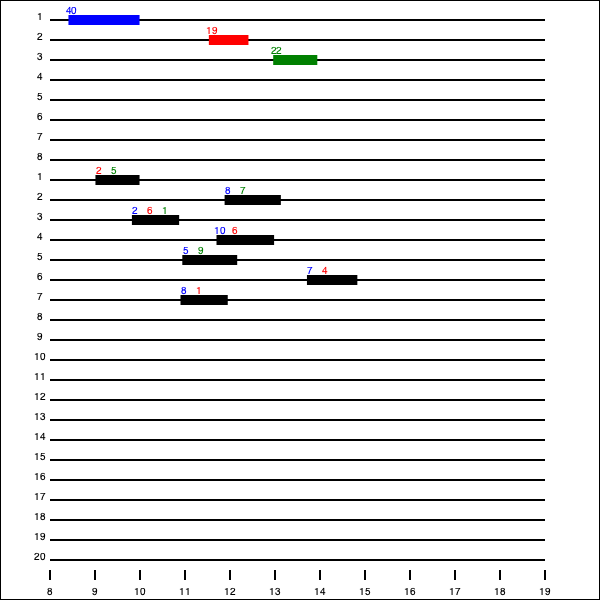
\includegraphics[scale=0.5]{images/TDAPplanning.png}
%\end{minipage}
%\begin{minipage}{0.5\textwidth}
\caption{Example of a planning. Timewindows for incoming trucks are on the top, where a color represents a given furnished, and the number indicates the number of pallets to deliver. Timewindows for outcoming trucks are on the bottom colored in black, where the colored number represents the number of pallets to collect from a given furnisher.}
\label{fig:planning}
%\end{minipage}
\end{figure}


A series of 10 "bi-partite" instances have been generated.

%
Note that in an operational solution, an incoming truck may leave the warehouse with pallets, if they cannot be transhipped through the crossdock to the corresponding outcoming trucks. The capacity problem discussed in Section \ref{sec:palletnotTransferred} does not exist in this configuration.


\newpage
%
% =======================================================================
%
\subsection{Experiments}

\color{red}
The goal of the experiments is not to put in competition the formulations since they handle different hypotheses (no temporary storage for M vs temporary storage for G; macroscopic view of pallet's flow plus aggregated single objective for M and G vs microscopic view of pallet's flow plus multiple objective without artifact costs for 2R), but to observe and understand the optimal solutions outputted by formulations.
\color{black}

%
% ===
%
\subsubsection{Experimental environment}

All the algorithms are implemented in Julia (version 1.10) and uses JuMP (version 1.21) as algebraic modeling language.
The codes are available online at \url{https://github.com/xgandibleux/TDAP}.
The experiment are performed on a  MacBook Pro laptop under macOS Ventura (version 13.6) equipped as follow:
\begin{itemize}
    \item CPU model: 3.5 GHz Intel Core i7 double cores.
    \item Memory: 16 Go 2133 MHz LPDDR3.
\end{itemize}
Gurobi Optimizer (version 10.0.3 build v10.0.3rc0 (mac64[x86]))  is used as MIP solver\footnote{The codes provided online are ready to use GLPK as MIP solver.}.  


%
% ===
%
\subsubsection{Experiment 1: comparison between formulations M and G}\label{sec:resMG}

This experiment focusses on  the optimal solutions obtained by the M and G formulations on small and medium size instances
 ``full mesh''.
%
In particular, we want to observe the pallets transferred between trucks.
%whether the formulation G is indeed capable of finding optimal solutions with a higher number of pallets transferred between trucks than the formulation M.
%
For this experiment, a computation time limit of 600 seconds is given to Gurobi\footnote{\citet{MIAO2009} have reported the difficulty for finding optimal solutions for medium-sized instances within a set time limit of 7200 seconds using CPLEX.}.
This value was chosen because it has shown to be sufficient to observe the behaviour of the two formulations given our computer configuration.

65 instances of increasing size were selected from the available dataset with the aim of being optimally solved by Gurobi.
% we will therefore selected instances manageab 600 seconds is appeared as the limit on our configuration}.%, which is not anymore true for the following instances available in the dataset. 
%
For both formulations and for each instance, the results collected, i.e. 
(1) the optimal objective value (aggregated cost, operational cost, penalty cost), 
(2) the CPUtime in seconds,
(3) the transferts of pallets between docks (number and percentage) achieved,   and
(4) the number of trucks assigned to a dock
are gathered together in Tables \ref{tab:M_results} and \ref{tab:G_results}, and Figures \ref{fig:res1MG} and \ref{fig:res2MG} synthesise  graphically these results.

\color{red}

%# commandes pour extraire les chiffres
%julia> for i in 1:nrow(dfM) if dfM[i,:tElapsed] < dfG[i,:tElapsed] println(i, " ", dfM[i,:fname], " ", dfM[i,:tElapsed], " ", dfG[i,:tElapsed]); end; end
%12 data_12_6_1 63.788 89.21
%13 data_12_6_2 176.614 191.381

Hormis pour deux instances de petites tailles, la figure \ref{fig:resTimeMG} montre que la formulation M requière plus de temps de resolution au solveur MIP que la formulation G.
L'écart entre les deux augmente significativement lorsque les tailles d'instance augmentent, notamment lorsque le nombre de docks à considérer augmente.
Le temps de resolution d'une instance sous la formulation M avec Gurobi atteint la limite de temps de 600 secondes bien avant la formulation G.
Sous l'angle des temps de resolution, la formulation G apparait donc meilleure que la formulation M.
Here, It is worth to remind that results are presented in \citep{Gelareh2015,GELAREH2016} to tighten the formulation G, letting a potential advantage to the latter formulation on this criterion.

%# commandes pour extraire les chiffres
%julia> for i in 1:nrow(dfM) if dfM[i,:zOpt] < dfG[i,:zOpt] && dfM[i,:zOpt] != -1 println(i, " ", dfM[i,:fname], " ", dfM[i,:zOpt], " ", dfG[i,:zOpt]); end; end
%6 data_12_4_0 13508 13554
%13 data_12_6_2 2251 2366
%15 data_12_6_4 2625 2809
%21 data_14_6_0 6254 6380
%30 data_16_4_4 9664 9951
%32 data_16_6_1 3485 3915

%# commandes pour extraire les chiffres
%julia> for i in 1:nrow(dfM) if dfM[i,:zOptCost] < dfG[i,:zOptCost] && dfM[i,:zOptCost] != -1 println(i, " ", dfM[i,:fname], " ", dfM[i,:zOptCost], " ", dfG[i,:zOptCost]); end; end

%# commandes pour extraire les chiffres
%julia> for i in 1:nrow(dfM) if dfM[i,:zOptPenalty] < dfG[i,:zOptPenalty] && dfM[i,:zOptPenalty] != -1 println(i, " ", dfM[i,:fname], " ", dfM[i,:zOptPenalty], " ", dfG[i,:zOptPenalty]); end; end
%1 data_10_3_0 3003 3067
%6 data_12_4_0 13312 13462
%13 data_12_6_2 1719 2106
%14 data_12_6_3 0 189
%15 data_12_6_4 2203 2623
%18 data_14_4_2 7096 7368
%21 data_14_6_0 5494 6088
%30 data_16_4_4 9378 9864
%32 data_16_6_1 2679 3622
%33 data_16_6_2 7618 7625
%37 data_18_4_1 1301 1629
%38 data_18_4_2 12486 12515
%41 data_18_6_0 5467 5651
%42 data_18_6_1 7664 7896
%44 data_18_6_3 9326 9736
%49 data_20_6_3 10021 10197

Comme le rapporte la figure \ref{fig:resObjFctMG}, la valeur optimale de la fonction économique obtenue avec la formulation G est inférieure a la valeur obtenue avec la formulation M, hormis pour six instances.
La faiblesse pointée par \citet{Gelareh2015} dans la formulation M et la correction proposée avec la formulation G apparait justifiée numériquement mais sans toutefois dominer sur toutes les instances.
En regardant de plus près les valeurs dans les tables \ref{tab:M_results} et \ref{tab:G_results}, c'est la partie cout opérationnel qui est plus élevée dans les solutions optimales obtenues avec la formulation M.
Par contre le cout de pénalité dans les solutions optimales apparait equivalent dans les deux formulations, avec une valeur légèrement à l'avantage de la formulation M pour 16 instances.
La formulation M élabore donc des solutions optimales avec un meilleur nombre de transfert, ce que illustrent les figures \ref{fig:resNbrTfsMG} et \ref{fig:resDiffTfsMG} qui rapportent le nombre de transferts de palettes réalisés dans les solutions optimales pour les deux formulations.
Ceci invalide numériquement l'affirmation qui avance que la formulation G  permet d'effectuer davantage de transferts de palettes que la formulation M. 
En effet, tres souvent les deux formulations donnent le même nombre de transfert comme le montre la figure \ref{fig:resDiffTfsMG}; et quand ce n'est pas le cas, la formulation M rapporte un nombre de transfert tres légèrement supérieur.

Vu d'un exploitant de terminal de cross-docking, cette nuance peut s'avérer sensible. 
En effet, il apparait raisonnable de souhaiter optimiser en première priorité le nombre de palettes transférées, et optimiser en seconde priorité l'utilisation du terminal en réduisant le temps passé par les palettes dans le terminal.
Une utilisation optimisée du terminal offre la possibilité d'anticiper le départ des camions des docks. 

Ces observations faites sur les résultats numériques issus des formulations M et G justifient la transition à l'elaboration de solutions optimales à l'aide de la formulation bi-objectif 2R proposée qui permet notamment de rapporter des solutions lexicographiquement optimales.


%\vspace{10mm}
%The results numerically confirm the assertions presented in \citep{Gelareh2015,Gelareh2021}. Indeed, for all the instances, the optimal value of the objective function is higher for formulation M than the formulation G, notably due to the extra transportation costs discussed in Section \ref{sec:extratransportationcosts} and a lower penality occuring in the solution since the optimal number of pallets transferred is higher for formulation G than the formulation M, since in formulation G the temporary storage in the crossdock is allowed as discussed in Section \ref{sec:temporary storage}.

%Although it is not a main topic here, the CPU times used by GUROBI are in the same orders of magnitude for both formulations (except for a few instances where the time measured with formulation G is significantly higher). 
 \color{black}
 
\begin{figure}[h!]
  \begin{center}
   \begin{subfigure}{1\textwidth}
      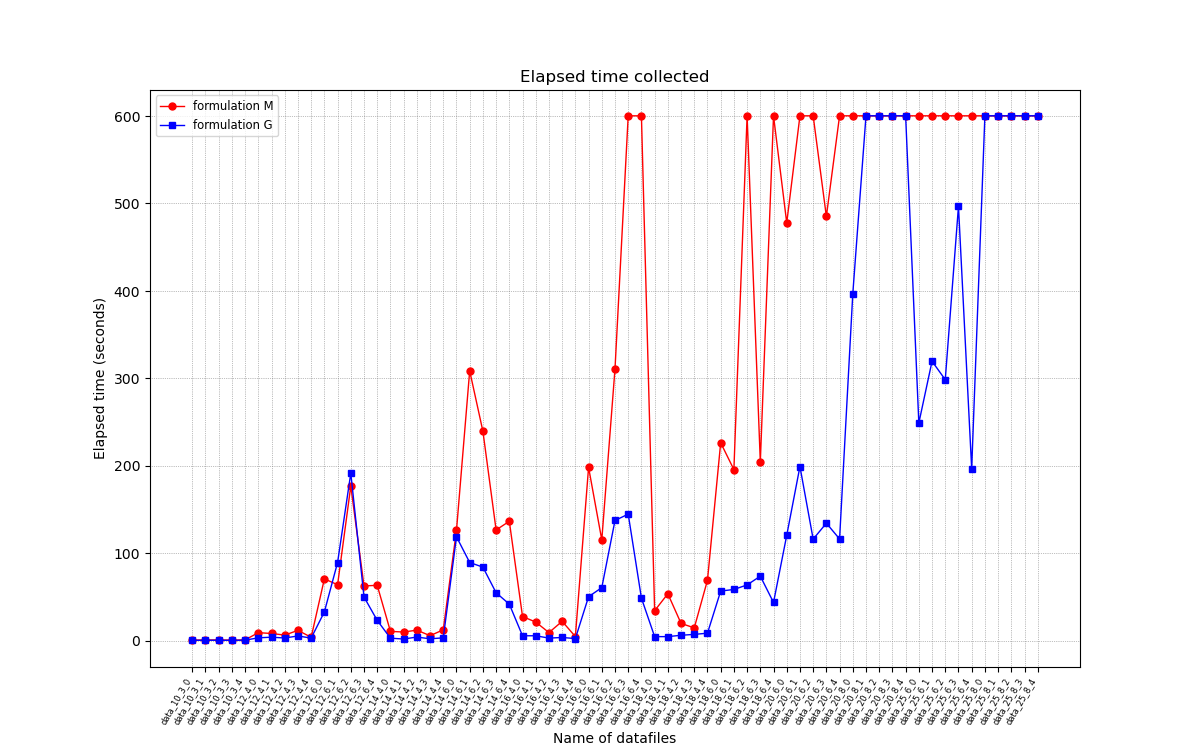
\includegraphics[scale=0.45]{images/resultsMGtime.png}
      \caption{Comparison elapsed time  collected for each instance. When a $y$ value is equal to 600, the corresponding optimal solution is not available.}
      \label{fig:resTimeMG}
    \end{subfigure}
    %
    \begin{subfigure}{1\textwidth}
      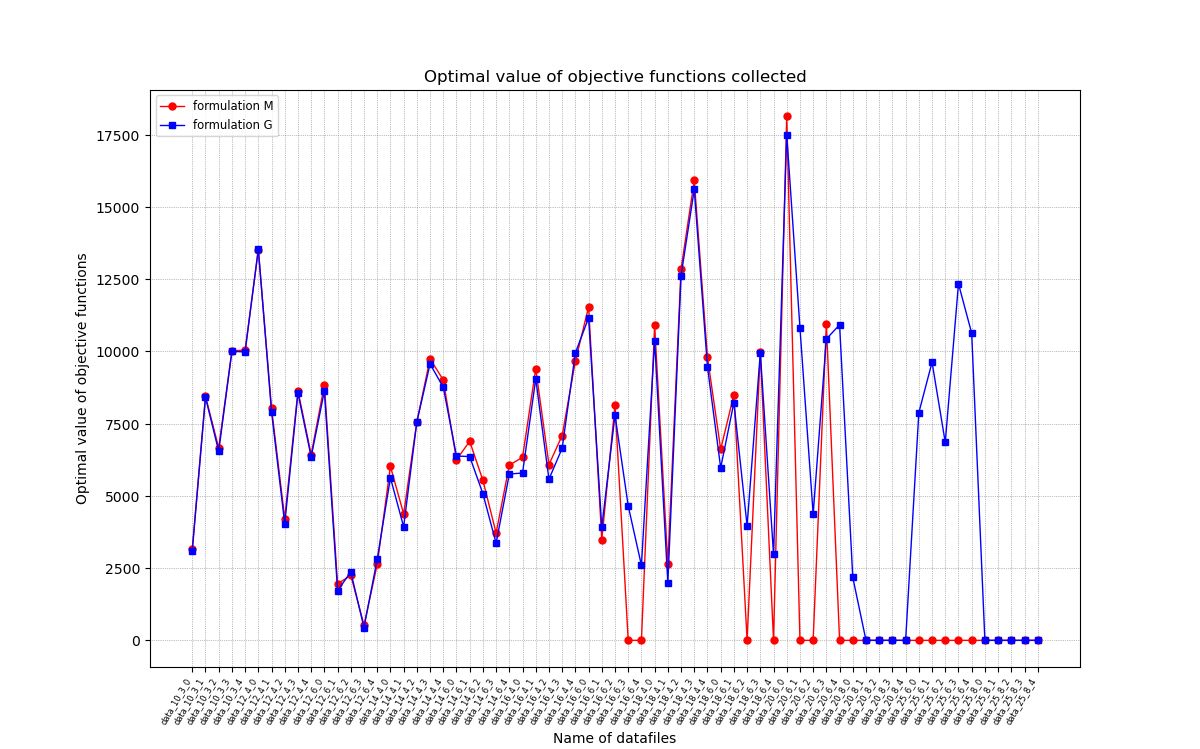
\includegraphics[scale=0.45]{images/resultsMGobjFct.png}
      \caption{Comparison of objective values collected for each instance. When a $y$ value is equal to 0, the corresponding optimal solution is not available.}
      \label{fig:resObjFctMG}
    \end{subfigure}
    %
  \end{center}
  \caption{Comparison between formulations M and G on the objective value and the elapsed time.}
   \label{fig:res1MG}
\end{figure}


\begin{figure}[h!]
  \begin{center}
    \begin{subfigure}{1\textwidth}
      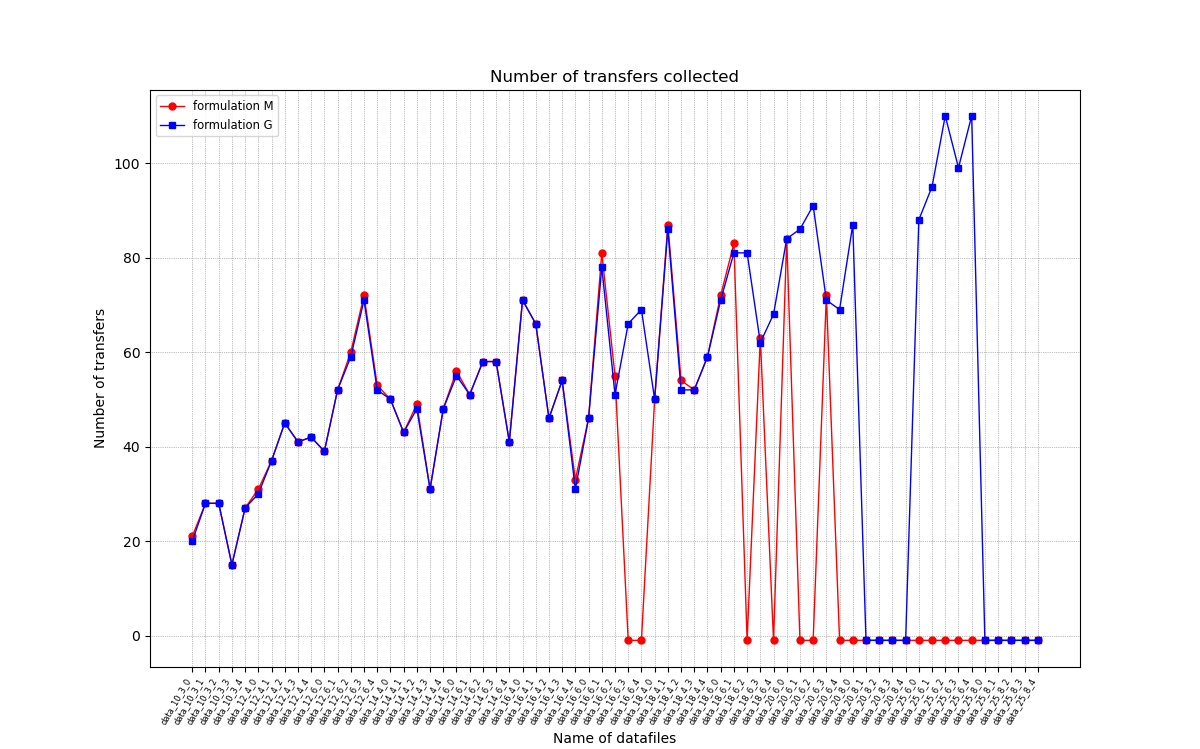
\includegraphics[scale=0.45]{images/resultsMGnbrTft.png}
      \caption{Comparison on number of transfers  collected for each instance. When a $y$ value is equal to 0, the corresponding optimal solution is not available.}
      \label{fig:resNbrTfsMG}
    \end{subfigure}
    %
    \begin{subfigure}{1\textwidth}
      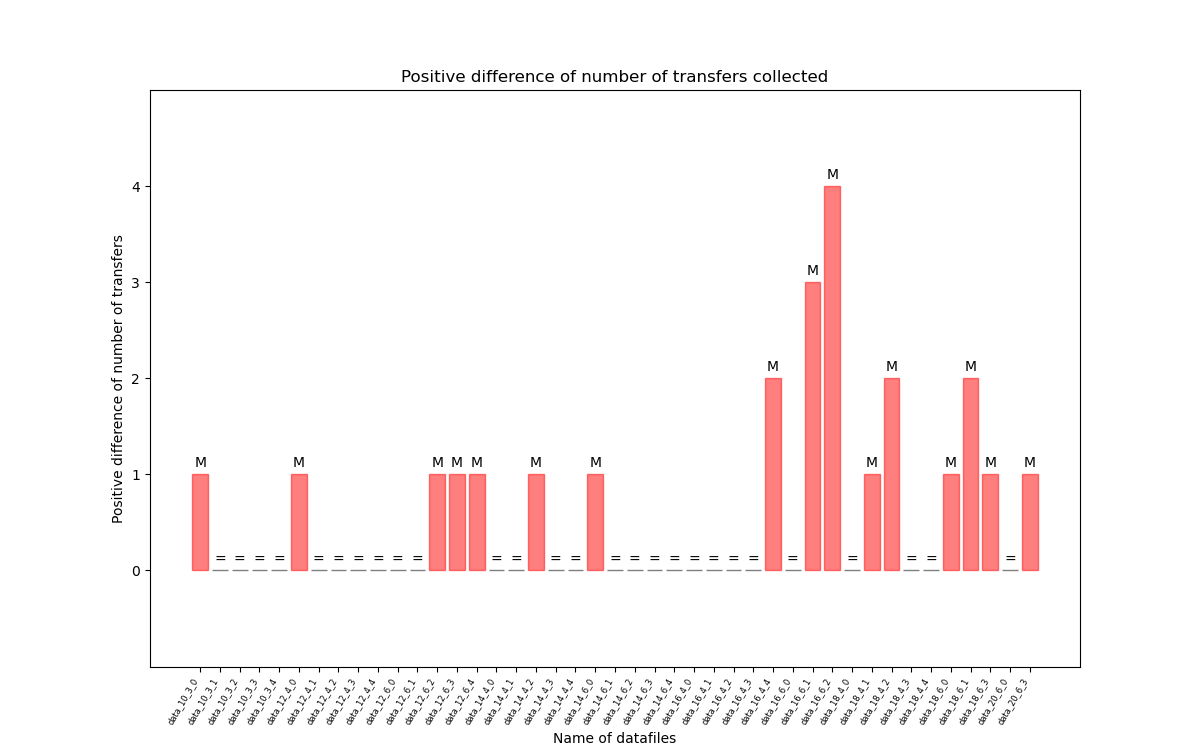
\includegraphics[scale=0.45]{images/resultsMGdifference.png}
      \caption{Positive difference on number of transfers  collected for each instance solved to optimality for both formulations. ``\texttt{M}'' means the difference is in favor of formulation M, ``\texttt{G}'' means the difference is in favor of formulation G,  ``\texttt{=}'' means there is no difference between the two formulations.}
      \label{fig:resDiffTfsMG}
    \end{subfigure}
    %
  \end{center}
  \caption{Comparison between formulations M and G on the number of transferts.}
   \label{fig:res2MG}
\end{figure}

%
% ===
%
\subsubsection{Experiment 2: results obtained with formulation 2R}\label{sec:res2R}

\color{red}
Expe a refaire, écriture à poursuivre
\color{black}

%
% =======================================================================
% =======================================================================
%
\section{Conclusion and perspectives} 
\label{sec:ConclusionPerspectives}

\color{red}
Ce papier se présente avant tout au lecteur comme un état de l’art synthétisant  les différents formulations qui sont rencontrées dans la littérature sur le TDAP depuis 2009. 
Les formulations, ici nommées M et G, sont décrites avec un cadre de notations unifiées, analysées et discutées.
%
Notre revue de la littérature mettra en évidence un certain nombre de points critiques/écueils relevés dans différentes papiers, engendrant notamment des publications de papiers  ayant pour objectif d'apporter une mise au point.
Alors que les auteurs concernés présentent un argumentaire et un fond technique solides, nous avons relevé différentes erreurs dans ces documents scientifiques publiés ou diffusés, pour lesquelles nous apportons présentement des corrections.
Ainsi notre premier volet de contribution à pour objectif de clarifier de manière rigoureuse les formulations des modèles IP décrivant le TDAP.

Notre second volet de contribution se décline en trois actes.
%
D'abord,  les discussions menée ont permis de mettre en lumière un certain nombre de points soit limitant, soit particularisant les formulations M et G.
Elles nous nous ont conduit à proposer une formulation 2R immédiatement dérivée de celles-ci, laquelle intègre une partie de ces points mis en lumière.
Ainsi cette formulation considère notamment deux fonctions objectif indépendamment et est plus fine dans la prise en compte des données au niveau des contraintes proposées.
%
Ensuite, les instances numériques utilisées dans les papiers relatifs aux formulations M et G questionnent également.
En réponse à cela, une nouvelle famille d’instance numérique a été proposé. Les fichiers de données et le générateur permettant de produire ces données sont disponibles en ligne en Open source à \url{https://github.com/xgandibleux/TDAP}.
%
Enfin, des expérimentations numériques sont rapportées.
Toutes les solutions produites par les trois modèles ont été obtenues avec un certificat d’optimalité.
Les méthodes et techniques de résolution utilisées pour calculer les solutions sont génériques. 
Implémentées en Julia et utilisant le langage de modélisation algébrique JuMP, la résolution des instances numériques présentée en entrée de l'une des trois formulations est obtenue avec le solveur GUROBI. Le package MOA qui propose une collection d'algorithmes multi-objectif est utilisé pour produire les solutions pour la formulation 2R. 

Les expérimentations numériques .... %illustrent et confirment quantitativement un certain nombre d’hypothèses avancées dans les discussions rapportées.

*** perspectives ***
\color{black}

%% -----------------------------------------------------------------------
%
%The following Table \ref{tab:synthesebib} summarizes the references support to our research work and the resolution approach proposed by the author's papers.
%
%\begin{table}[h!]
%\begin{center}
%\begin{tabular}{ |p{4.5cm}||p{7.5cm}|p{6cm}|}
% %\hline
% %\multicolumn{4}{|c|}{} \\
% \hline
%  & & \\
% References & Authors & Resolution approach \\
%  & & \\
% \hline
% & & \\
%  \citep{Lim2005,Lim2006} & A. Lim, H. Ma, Z. Miao         & Simulated Annealing     \\
%  \citep{MIAO2009}        & Z. Miao, A. Lim, H. Ma        & IP/Tabu Search/Genetic Algorithm \\
%   \citep{Gelareh2015}     & S. Gelareh, G. Goncalves, R. Monemi  &  Correction, new IP    \\
%  \citep{GELAREH2016}     & S. Gelareh, R. Monemi, F. Semet, G. Goncalves  & Branch\&Cut    \\
%  \citep{Daquin2021}      & C. Daquin, H. Allaoui, G. Goncalves, T. Hsu    & Variable Neighborhood Search     \\
%  \citep{Gelareh2021}     & S. Gelareh         &  Correction     \\
%  & & \\
% \hline
%\end{tabular}
%\end{center}
%\caption{Timeline and key information about the major contributions considered in this paper.}
%\label{tab:synthesebib}
%\end{table}%




%\newpage
%%
%% =======================================================================
%% =======================================================================
%%
%
%%% Use \section commands to start a section
%\section{Example Section}
%\label{sec1}
%%% Labels are used to cross-reference an item using \ref command.
%
%Section text. See Subsection \ref{subsec1}.
%
%%% Use \subsection commands to start a subsection.
%\subsection{Example Subsection}
%\label{subsec1}
%
%Subsection text.
%
%%% Use \subsubsection, \paragraph, \subparagraph commands to 
%%% start 3rd, 4th and 5th level sections.
%%% Refer following link for more details.
%%% https://en.wikibooks.org/wiki/LaTeX/Document_Structure#Sectioning_commands
%
%\subsubsection{Mathematics}
%%% Inline mathematics is tagged between $ symbols.
%This is an example for the symbol $\alpha$ tagged as inline mathematics.
%
%%% Displayed equations can be tagged using various environments. 
%%% Single line equations can be tagged using the equation environment.
%\begin{equation}
%f(x) = (x+a)(x+b)
%\end{equation}
%
%%% Unnumbered equations are tagged using starred versions of the environment.
%%% amsmath package needs to be loaded for the starred version of equation environment.
%\begin{equation*}
%f(x) = (x+a)(x+b)
%\end{equation*}
%
%%% align or eqnarray environments can be used for multi line equations.
%%% & is used to mark alignment points in equations.
%%% \\ is used to end a row in a multiline equation.
%\begin{align}
% f(x) &= (x+a)(x+b) \\
%      &= x^2 + (a+b)x + ab
%\end{align}
%
%\begin{eqnarray}
% f(x) &=& (x+a)(x+b) \nonumber\\ %% If equation numbering is not needed for a row use \nonumber.
%      &=& x^2 + (a+b)x + ab
%\end{eqnarray}
%
%%% Unnumbered versions of align and eqnarray
%\begin{align*}
% f(x) &= (x+a)(x+b) \\
%      &= x^2 + (a+b)x + ab
%\end{align*}
%
%\begin{eqnarray*}
% f(x)&=& (x+a)(x+b) \\
%     &=& x^2 + (a+b)x + ab
%\end{eqnarray*}
%
%%% Refer following link for more details.
%%% https://en.wikibooks.org/wiki/LaTeX/Mathematics
%%% https://en.wikibooks.org/wiki/LaTeX/Advanced_Mathematics
%
%%% Use a table environment to create tables.
%%% Refer following link for more details.
%%% https://en.wikibooks.org/wiki/LaTeX/Tables
%\begin{table}[t]%% placement specifier
%%% Use tabular environment to tag the tabular data.
%%% https://en.wikibooks.org/wiki/LaTeX/Tables#The_tabular_environment
%\centering%% For centre alignment of tabular.
%\begin{tabular}{l c r}%% Table column specifiers
%%% Tabular cells are separated by &
%  1 & 2 & 3 \\ %% A tabular row ends with \\
%  4 & 5 & 6 \\
%  7 & 8 & 9 \\
%\end{tabular}
%%% Use \caption command for table caption and label.
%\caption{Table Caption}\label{fig1}
%\end{table}


\clearpage
\newpage
%
% =======================================================================
% =======================================================================
%
%% The Appendices part is started with the command \appendix;
%% appendix sections are then done as normal sections
\appendix

\section{Formulation G  from \citet{Gelareh2015,GELAREH2016,Gelareh2021}}
\label{app:formulationsG}

%
% =======================================================================
%
\subsection{The original formulation}
\label{app:formulationsGoriginale}
\medskip

The decision variables are identical to the formulation M (see Section \ref{sec:FormulationM}).
%
The IP model is thus formulated as (reproduced exactly as presented in papers, with errors and missing information): \\
    \begin{equation*}
    \begin{array}{ll@{}ll}
    \text{min}  & \displaystyle\sum\limits^{m}_{k=1} \sum^{m}_{l=1} \sum^{n}_{i=1} \sum^{n}_{j=1} c_{kl} \, t_{kl} \, z_{ijk} \ + \ \sum^{n}_{i=1}\left( \sum^{n}_{j=1} p_{ij} \, f_{ij} \left( 1-\sum^{m}_{k=1} \sum^{m}_{l=1} z_{ijkl} \right) \right) & \  (1) \vspace{2mm}\\
    \text{s.t.}     & \displaystyle\sum\limits^{m}_{k=1} y_{ik} \leq 1  \hfill  \forall i & \ (2)\vspace{2mm}\\
                    & z_{ijkl} \leq y_{ik}  \hfill  \forall i,j,k,l & \ (3)\vspace{2mm}\\
                    & z_{ijkl} \leq y_{jl}   \hfill  \forall i,j,k,l & \ (4) \vspace{2mm}\\
                    & y_{ik} + y_{jk} \leq 1 + \hat{x}_{ij} + \hat{x}_{ji}   \hfill   \forall i,j,k & \ (5) \vspace{2mm}\\
                    & z_{ijkk} \leq \hat{x}_{ij}   \hfill  \forall i,j \neq i,k,l & \ (6) \vspace{2mm}\\
                    & \displaystyle\sum\limits_{k=1}^{m} \sum_{l=1}^{m} \sum_{i\in\{i:a_{i} \le \tau_r\}} \sum_{j=1}^{n} f_{ij} \, z_{ijkl} \ + \ \sum_{k=1}^{m} \sum_{l=1}^{m} \sum_{i}^{n} \sum_{j\in\{j:d_{j} \le \tau_r\}} f_{ij} \, z_{ijkl} \le  C \hspace{0.25cm} \hfill \forall r \in \{1,2,...,2n\} & \ (7) \vspace{2mm}\\ 
                    & z_{ijkl} = 0  \hfill  \forall i,j,k,l : j \neq i, (d_j - a_i - t_{kl} \leq 0) & \ (8) \vspace{2mm}\\
                    & z_{ijkl} \le 1   \hfill  \forall i,j,k,l : j \neq i & \ (9) \vspace{2mm}\\ 
                    & z_{ijkl} \ge 0   \hfill  \forall i,j,k,l : j \neq i &  \ (10) \vspace{2mm}\\ 
                    & y_{ik} \le 1   \hfill  \forall i,k & \ (11) \vspace{2mm}\\ 
                    & y_{ik} \ge 0 \hfill  \forall i,k &  \ (12) \vspace{2mm}\\                     
                    & y_{ik} \in \{0,1\}, \ z_{ijkl} \in \{0,1\} &  \ (13) \vspace{2mm}
    \end{array}
    \end{equation*}
%\smallskip

\vspace{-2mm}
\noindent
where:
\begin{itemize}
    \item [(5)] guarantee that if the arrival/departure time windows of two trucks $i$ and $j$ overlap ($\hat{x}_{ij} = \hat{x}_{ji}=0$), either of them can be docked at dock $k$ (not both);
    \item [(6)] ensure that truck $i$ and truck $j$ can use the same dock for realizing the transfers of pallets from $i$ to $j$, only if their time windows do not intersect (i.e. $i$ leaves no later than $j$ arrives); 
    \item [(8)] ensure that $z_{ijkl}$ is set to zero if $f_{ij}>0$ and $(d_j - a_i - t_{kl} < 0)$.
\end{itemize}
and the others parts of the formulation (i.e. (1-4), (7), and (13)) share the same definition with the formulation M.  

%
% =======================================================================
%
\subsection{The corrections proposed}
\label{app:CorrectionsG}
\medskip

A number of inaccuracies and incompleteness were identified in formulation G, making this formulation non-operational. Because of this we were unable to reproduce the results announced by the authors. They are reported hereafter (also coloured in red in the text).

  \begin{itemize}
      \item [--] in (1): index missing into the first term:       \vspace{2mm} \\
      $\displaystyle\sum\limits^{m}_{k=1} \sum^{m}_{l=1} \sum^{n}_{i=1} \sum^{n}_{j=1} c_{kl} \, t_{kl} \, z_{ijk{\color{red}l}} \ + \ \sum^{n}_{i=1}\left( \sum^{n}_{j=1} p_{ij} \, f_{ij} \left( 1-\sum^{m}_{k=1} \sum^{m}_{l=1} z_{ijkl} \right) \right)$
      \vspace{2mm}

      \item [--] in (5): wrong definition of index:       \vspace{2mm} \\
      $y_{ik} + y_{jk} \leq 1 + \hat{x}_{ij} + \hat{x}_{ji} \hspace{64.5mm} \forall i,j \color{red}\neq i \color{black},k$
      \vspace{2mm}      
      
      \item [--] in (6):  wrong definition of index:       \vspace{2mm} \\
      $z_{ijkk} \leq \hat{x}_{ij} \hspace{86mm} \forall i,j \neq i,k,\color{red}{l}\color{black}$
      \vspace{2mm}

      \item [--] in (7):  wrong operation, and initial value missing:       \vspace{2mm} \\
      $\displaystyle\sum\limits_{k=1}^{m} \sum_{l=1}^{m} \sum_{i\in\{i:a_{i} \le \tau_r\}} \sum_{j=1}^{n} f_{ij} \, z_{ijkl} \ \color{red}{-}\color{black} \ \sum_{k=1}^{m} \sum_{l=1}^{m} \color{red}\sum_{i=1}^{n}\color{black} \sum_{j\in\{j:d_{j} \le \tau_r\}} f_{ij} \, z_{ijkl} \le  C \hspace{1mm} \quad \forall r \in \{1,2,...,2n\}$
      \vspace{2mm}

      \item [--] in (9-12):  constraints (9-12) redundant with (13), and domains of indexes not stated in (13):       \vspace{2mm} \\
      $y_{ik} \in \{0,1\}, \ z_{ijkl} \in \{0,1\}$
      \vspace{2mm}
  \end{itemize}
 
Taken individually each of these points can be corrected quite easily once identified. 
%
However, some are not immediately identifiable, as in the case of the point relating to constraint (5), which could only be identified after a meticulous analysis of the flat formulation, which necessitated testing instances by hand.


\section{Formulations implemented in Julia with JuMP}
\label{app:formulations}

%
% =======================================================================
%
\subsection{Formulation M}
\label{app:JuMPformulationM}

{\scriptsize
\begin{verbatim}

using JuMP
mod = Model()

# --- Variables ---------------------------------------------------------------
# 1 if truck i is assigned to dock k, 0 otherwise: 
@variable( mod, 
           y[1:n, 1:m], Bin
         )
# 1 if truck i is assigned to dock k and truck j to dock l, 0 otherwise:
@variable( mod, 
           z[1:n, 1:n, 1:m, 1:m], Bin
         )
         
# --- (1): objective ----------------------------------------------------------
# total operational cost + total penalty cost:
@objective( mod, 
            Min, 
            sum(c[k,l] * t[k,l] * z[i,j,k,l] for i=1:n, j=1:n, k=1:m, l=1:m)
            +
            sum( (sum( p[i,j] * f[i,j] * ( 1 - sum( z[i,j,k,l] for k=1:m, l=1:m) ) for j=1:n) ) for i=1:n)
          )
          
# --- (2-8): constraints ------------------------------------------------------
@constraint( mod, 
             cst2_[i=1:n], 
             sum(y[i,k] for k=1:m) <= 1
           ) 
@constraint( mod, 
             cst3_[i=1:n, j=1:n, k=1:m, l=1:m], 
             z[i,j,k,l] <= y[i,k]
           )
@constraint( mod, 
             cst4_[i=1:n, j=1:n, k=1:m, l=1:m], 
             z[i,j,k,l] <= y[j,l]
           )
@constraint( mod, 
             cst5_[i=1:n, j=1:n, k=1:m, l=1:m], 
             y[i,k] + y[j,l] - 1 <= z[i,j,k,l]
           )
@constraint( mod, 
             cst6_[i=1:n, j=1:n, k=1:m; i!=j], 
             x[i,j] + x[j,i] >= z[i,j,k,k]
           )
@constraint( mod, 
             cst7_[r=1:2*n], 
             sum(f[i,j] * z[i,j,k,l] for i in atr[r], j=1:n, k=1:m, l=1:m)
             - 
             sum(f[i,j] * z[i,j,k,l] for i=1:n, j in dtr[r], k=1:m, l=1:m) <= C
           )
@constraint( mod, 
             cst8_[i=1:n, j=1:n, k=1:m, l=1:m], 
             f[i,j] * z[i,j,k,l] * (d[j] - a[i] - t[k,l]) >= 0
           )
\end{verbatim}
}


%
% =======================================================================
%
\subsection{Formulation G after having fixed issues}
\label{app:JuMPformulationG}

{\scriptsize
\begin{verbatim}

using JuMP
mod = Model()

# --- Variables ---------------------------------------------------------------
# 1 if truck i is assigned to dock k, 0 otherwise: 
@variable( mod, 
           y[1:n, 1:m], Bin
         )
# 1 if truck i is assigned to dock k and truck j to dock l, 0 otherwise:
@variable( mod, 
           z[1:n, 1:n, 1:m, 1:m], Bin
         )

# --- (1): objective ----------------------------------------------------------
# total operational cost + total penalty cost
@objective( mod, 
            Min, 
            sum(c[k,l] * t[k,l] * z[i,j,k,l] for i=1:n, j=1:n, k=1:m, l=1:m)
            +
            sum( (sum( p[i,j] * f[i,j] * ( 1 - sum( z[i,j,k,l] for k=1:m, l=1:m) ) for j=1:n) ) for i=1:n)
          )

# --- (2-8): constraints ------------------------------------------------------
@constraint( mod, 
             cst2_[i=1:n], 
             sum(y[i,k] for k=1:m) <= 1
           ) 
@constraint( mod, 
             cst3_[i=1:n, j=1:n, k=1:m, l=1:m], 
             z[i,j,k,l] <= y[i,k]
           )
@constraint( mod, 
             cst4_[i=1:n, j=1:n, k=1:m, l=1:m], 
             z[i,j,k,l] <= y[j,l]
           )
@constraint( mod, 
             cst5_[i=1:n, j=1:n, k=1:m; i!=j], 
             y[i,k] + y[j,k] <= 1 + x[i,j] + x[j,i]
           )
@constraint( mod, 
             cst6_[i=1:n, j=1:n, k=1:m; i!=j],
             z[i,j,k,k] <= x[i,j] 
           )
@constraint( mod, 
             cst7_[r=1:2*n], sum(f[i,j] * z[i,j,k,l] for i in atr[r], j=1:n, k=1:m, l=1:m)
             - 
             sum(f[i,j] * z[i,j,k,l] for i=1:n, j in dtr[r], k=1:m, l=1:m) <= C
           )
@constraint( mod, 
             cst8_[i=1:n, j=1:n, k=1:m, l=1:m; i!=j && (d[j]-a[i]-t[k,l])<=0],  
             z[i,j,k,l] == 0
           )
\end{verbatim}
}


%\newpage
%%
%% =======================================================================
%%
%\subsection{Formulation R}
%\label{app:JuMPformulationR}
%
%{\scriptsize
%\begin{verbatim}
%
%using JuMP
%mod = Model()
%
%# --- Variables ---------------------------------------------------------------
%# 1 if truck i is assigned to dock k, 0 otherwise: 
%@variable( mod, 
%           y[1:n, 1:m], Bin
%         )
%# 1 if truck i is assigned to dock k and truck j to dock l, 0 otherwise:
%@variable( mod, 
%           z[1:n, 1:n, 1:m, 1:m], Bin
%         )
%         
%# --- (1): objective ----------------------------------------------------------
%# total operational cost + total penalty cost
%@objective( mod, 
%            Min, 
%            sum(c[k,l] * t[k,l] * z[i,j,k,l] for i=1:n, j=1:n, k=1:m, l=1:m)
%            +
%            sum( (sum( p[i,j] * f[i,j] * ( 1 - sum( z[i,j,k,l] for k=1:m, l=1:m) ) for j=1:n) ) for i=1:n)
%          )
%          
%# --- (2-8): constraints ------------------------------------------------------
%@constraint( mod, 
%             cst2_[i=1:n], 
%             sum(y[i,k] for k=1:m) <= 1
%           ) 
%@constraint( mod, 
%             cst3_[i=1:n, j=1:n, k=1:m, l=1:m], 
%             z[i,j,k,l] <= y[i,k]
%           )
%@constraint( mod, 
%             cst4_[i=1:n, j=1:n, k=1:m, l=1:m], 
%             z[i,j,k,l] <= y[j,l]
%           )
%@constraint( mod, 
%             cst5_[i=1:n, j=1:n, k=1:m; i!=j], 
%             y[i,k] + y[j,k] <= 1 + x[i,j] + x[j,i]
%           )
%@constraint( mod, 
%             cst6_[i=1:n, j=1:n, k=1:m; i!=j],
%             z[i,j,k,k] <= x[i,j]
%           )
%@constraint( mod, 
%             cst7_[r=1:2*n], 
%             sum(f[i,j] * z[i,j,k,l] for i in atr[r], j=1:n, k=1:m, l=1:m)
%             - 
%             sum(f[i,j] * z[i,j,k,l] for i=1:n, j in dtr[r], k=1:m, l=1:m) <= C
%           )
%@constraint( mod, 
%             cst8_[i=1:n, j=1:n, k=1:m, l=1:m; i!=j && (d[j]-a[i]-f[i,j]*t[k,l])<=0],  
%             z[i,j,k,l] == 0
%           )
%\end{verbatim}
%}


%
% =======================================================================
%
\subsection{Formulation 2R}
\label{app:JuMPformulation2R}

Code

\newpage

%
% =======================================================================
%
\subsection{Considerations for Generating Bipartite Instances}
\label{app:ConsiderationsInstancesBipartite}

\bigskip
\noindent
$\bullet$ \textit{The crossdock.}\\
%
A real warehouse has been choosen as reference. 
%It is one equiment from the Cargomatic company,  located near Laval (32 rue Bernard Palissy F53960 Bonchamp).
Built on a surface of $42 \times 20$ meters, the crossdock has a layout of ``I'' and presents 14 docks.


The distances between docks is based on the Manhattan distance between two docks. Measures are deduced from the physical configuration of the warehouse.

The crossdock has no fix equipment inside. It is viewed as an empty building where the pallets are transfered by forklifts.

If any pallets have to be temporary stored, they remain located on the area near the dock where the incoming truck has delivered these pallets.


\bigskip
\noindent
$\bullet$ \textit{Maximal number of pallets in a truck.}\\
%
A standard pallet has a surface of $120 cm \times 80 cm$ in general.
%
The maximum number of pallets transported by a truck depends of the type of truck. According the specialised website\footnote{\url{https://www.transports64.fr/combien-de-palette-dans-un-camion}}, the number of transported pallets is given in Table~\ref{tab:nbPalettes}.


\begin{table}[h!]
\begin{center}
\begin{tabular}{|c|c|}
\hline
\quad Number of wheels of the truck \quad & \quad Number of standard pallets $\mbox{  }$\quad \\
\hline
6 wheels (three-axle truck) & 14 to 16 standard pallets \\
10 wheels (five-axle truck) & 24 to 30 standard pallets \\
12-wheel truck (six-axle truck)& 36 to 40 standard pallets \\
16 wheels & 48 to 56 standard pallets\\
\hline
\end{tabular}
\caption{Number of pallets transported by a truck.}
\label{tab:nbPalettes}
\end{center}
\end{table}%


\noindent
$\bullet$ \textit{Loading/unloading a truck.}\\
%
In average, 1 minute is required to loading/unloading a pallet in a truck with a forklift.
%
Also 15 minutes are legaly required in France for completing various operations (coupling the truck at the dock, fulfill the administrative procedure, and the control of cargo).


\bigskip
\noindent
$\bullet$ \textit{The forklifts.}\\
% 
Inside a warehouse or a factory, the French reglementation limits the forklift speed to maximum 10km/h\footnote{\url{https://www.boplan.com/fr/les-reglementations-circulation-des-chariots-elevateurs}}.
%
In practice, the speed is much more low for security reasons and to protect the cargo during the transfer of pallets.

Knowing now the distance between docks and the speed of a forklift, a time $t_{kl}$ required for transfering one pallet between two docks is computed.


\bigskip
\noindent
$\bullet$ \textit{Incoming/outcoming trucks.}\\
%
We call ``incoming trucks'', those who carry pallets issued from furnishers (factories, other warehouses, etc.), and outcoming trucks, those who carry pallets to customers (shops, other warehouses, etc.).

We consider the capacity of incoming trucks larger than the outcoming ones. Also incoming trucks do not receive pallets from any other trucks. Only outcoming trucks receive pallets. Thus the transfer of pallets can be seen following a bi-partite graph (see Figure \ref{fig:fluxbiparti}), giving the name of this new collection. 

Note that an incoming truck may leave the warehouse with pallets, if they cannot be transhipped through the crossdock to the corresponding outcoming trucks.
The capacity problem discussed in Section \ref{sec:palletnotTransferred} does not exist in this configuration.


\newpage


%
% =======================================================================
%
\subsection{Results for formulations M and G}
\label{app:ResultatsMG}

%Table \ref{tab:M_vs_G_results} gives a comparison of results between formulations M and G

%\begin{table}[h!]
%  \hspace{1.5cm}
%  \vspace{0.5cm}
%  \centering
%{\scriptsize
%        \begin{tabular}{|c||c|c|c||c|c|c|}
%            \cline{2-7}
%             \multicolumn{1}{c|}{} & \multicolumn{3}{|c||}{Formulation M} & \multicolumn{3}{c|}{Formulation G} \\
%             \hline
%            Instances  & ObjValue & CPUtime (s) & \#Transfers  & ObjValue & CPUtime (s) & \#Transfers \\ 
%            \hline
%10\_3\_0 &  6363 &     1.030 &        9 		&  4880 &     1.318 &       14 \\
%10\_3\_1 & 16198 &     0.038 &        6 		& 14539 &     0.095 &       11 \\
%10\_3\_2 & 12143 &     0.052 &        9 		& 10875 &     0.233 &       12 \\
%\hline
%12\_4\_0 & 20914 &     0.193 &        6 		& 18468 &     0.456 &       11 \\
%12\_4\_1 & 17960 &     0.387 &        7 		& 14039 &     0.557 &       17 \\
%12\_4\_2 & 15945 &     0.401 &        8 		& 12263 &     0.553 &       18 \\
%12\_6\_0 & 18291 &     0.855 &        7 		& 16211 &     1.293 &       14 \\
%12\_6\_1 & 13769 &     1.157 &        6 		&  9510 &     1.693 &       19 \\
%12\_6\_2 & 18429 &     0.668 &        3 		& 13123 &     0.879 &       18 \\
%\hline
%14\_4\_0 & 18574 &     1.445 &        7 		& 12909 &     0.899 &       25 \\
%14\_4\_1 & 13829 &     1.449 &       13 		&  8918 &     1.266 &       25 \\
%14\_4\_2 & 17901 &     0.770 &       14 		& 14925 &     1.393 &       24 \\
%14\_6\_0 & 21707 &     3.315 &        7 		& 16753 &     2.046 &       21 \\
%14\_6\_1 & 18899 &     1.912 &        7 		& 14276 &     1.308 &       21 \\
%14\_6\_2 & 20533 &     2.227 &        6 		& 15794 &     2.197 &       18 \\
%\hline
%16\_4\_0 & 23990 &     3.287 &       13 		& 15373 &     2.407 &       38 \\
%16\_4\_1 & 24447 &     1.440 &       13 		& 18493 &     1.672 &       31 \\
%16\_4\_2 & 18294 &     1.864 &        8 		& 14532 &     0.917 &       23 \\
%16\_6\_0 & 22735 &     1.661 &       12 		& 19118 &     2.211 &       19 \\
%16\_6\_1 & 25353 &     5.745 &        7 		& 17515 &     5.547 &       30 \\
%16\_6\_2 & 21905 &     2.072 &        9 		& 17724 &     2.271 &       21 \\
%\hline
%18\_4\_0 & 21282 &     1.994 &       18 		& 15132 &     1.914 &       35 \\
%18\_4\_1 & 20692 &     2.251 &       12 		& 11332 &     2.883 &       44 \\
%18\_4\_2 & 25881 &     1.231 &       14 		& 21227 &     1.770 &       29 \\
%18\_6\_0 & 24915 &     4.251 &       11 		& 19133 &     5.355 &       28 \\
%18\_6\_1 & 32609 &     7.860 &        9 		& 25762 &     9.684 &       32 \\
%18\_6\_2 & 26472 &     4.662 &       10 		& 19226 &     5.826 &       31 \\
%\hline
%20\_6\_0 & 42740 &     8.304 &        9 		& 34005 &    10.718 &       38 \\
%20\_6\_1 & 34333 &    13.353 &       10 		& 25639 &    23.567 &       38 \\
%20\_6\_2 & 27743 &     8.626 &       12 		& 18694 &    15.630 &       37 \\
%20\_8\_0 & 24744 &     8.042 &        8 		& 18072 &    20.371 &       30 \\
%20\_8\_1 & 31871 &    16.987 &       11 		& 24040 &   104.488 &       35 \\
%20\_8\_2 & 27822 &    23.785 &        9 		& 20324 &    52.347 &       32 \\
%\hline
%25\_6\_0 & 30570 &    33.979 &       14 		& 21240 &    15.393 &       42 \\
%25\_6\_1 & 33874 &    34.386 &       18 		& 22701 &    39.297 &       48 \\
%25\_6\_2 & 38473 &    23.276 &       14 		& 26005 &    83.644 &       47 \\
%25\_8\_0 & 31322 &    67.869 &       20 		& 22090 &  1009.776 &       46 \\
%25\_8\_1 & 36180 &    84.203 &       10 		& 27835 &    91.959 &       32 \\
%25\_8\_2 & 40509 &    79.604 &       13 		& 29523 &   174.266 &       41 \\
%\hline
%30\_6\_0 & 33621 &    33.383 &       22 		& 22824 &    15.567 &       56 \\
%30\_6\_1 & 38746 &    45.391 &       22 		& 26037 &    98.530 &       60 \\
%30\_6\_2 & 38578 &    49.607 &       19 		& 23759 &    50.611 &       64 \\
%30\_8\_0 & 42964 &   108.180 &      17 		& 31307 &   329.787 &       59 \\
%30\_8\_1 & 43888 &   111.697 &       21 		& 29313 &  2603.717 &       60 \\
%30\_8\_2 & 44768 &   229.062 &      16 		& 29750 &   649.032 &       64 \\
%%
%%35\_8\_0 & 42243 $^*$             &  $\geq$ 2700 &       26 		& 32230 &   261.887 &       51 \\
%%35\_8\_1 & 54379 &  1034.155 &       26 		& 39102 &   623.569 &       68 \\
%%35\_8\_2 & 49087 $^*$              &  $\geq$ 2700 &       22 		& 35708 &   729.574 &       60 \\
%\hline
%        \end{tabular}
%        }
%        \caption{Comparison of results between formulations M and G}
%    \label{tab:M_vs_G_results}
%\end{table}


\begin{table}[h!]
  \hspace{1.5cm}
  \vspace{0.5cm}
  \centering
{\tiny
\begin{tabular}{rrrrrrrr}
  \hline
  \textbf{fname} & \textbf{tElapsed} & \textbf{zOpt} & \textbf{zOptCost} & \textbf{zOptPenalty} & \textbf{nTransfertDone} & \textbf{nTruckAssigned} & \textbf{pTransfertDone} \\
  \texttt{ } & \texttt{sec} & \texttt{ } & \texttt{ } & \texttt{ } & \texttt{\#} & \texttt{\#} & \texttt{\%} \\\hline
  data\_10\_3\_0 & 0.53 & 3163 & 160 & 3003 & 21 & 9 & 67.74 \\
  data\_10\_3\_1 & 0.575 & 8454 & 156 & 8298 & 28 & 7 & 46.67 \\
  data\_10\_3\_2 & 0.691 & 6659 & 234 & 6425 & 28 & 8 & 58.33 \\
  data\_10\_3\_3 & 0.403 & 10021 & 60 & 9961 & 15 & 6 & 31.25 \\
  data\_10\_3\_4 & 0.723 & 10047 & 192 & 9855 & 27 & 7 & 45.76 \\
  data\_12\_4\_0 & 8.994 & 13508 & 196 & 13312 & 31 & 8 & 41.89 \\
  data\_12\_4\_1 & 8.036 & 8035 & 220 & 7815 & 37 & 9 & 56.06 \\
  data\_12\_4\_2 & 6.188 & 4215 & 344 & 3871 & 45 & 10 & 76.27 \\
  data\_12\_4\_3 & 11.606 & 8642 & 208 & 8434 & 41 & 9 & 59.42 \\
  data\_12\_4\_4 & 3.697 & 6429 & 198 & 6231 & 42 & 9 & 66.67 \\
  data\_12\_6\_0 & 70.511 & 8845 & 406 & 8439 & 39 & 9 & 57.35 \\
  data\_12\_6\_1 & 63.788 & 1954 & 408 & 1546 & 52 & 11 & 89.66 \\
  data\_12\_6\_2 & 176.614 & 2251 & 532 & 1719 & 60 & 11 & 89.55 \\
  data\_12\_6\_3 & 62.408 & 528 & 528 & 0 & 72 & 12 & 100.0 \\
  data\_12\_6\_4 & 63.126 & 2625 & 422 & 2203 & 53 & 11 & 88.33 \\
  data\_14\_4\_0 & 10.426 & 6023 & 684 & 5339 & 50 & 11 & 75.76 \\
  data\_14\_4\_1 & 9.734 & 4376 & 600 & 3776 & 43 & 12 & 78.18 \\
  data\_14\_4\_2 & 11.841 & 7568 & 472 & 7096 & 49 & 11 & 62.82 \\
  data\_14\_4\_3 & 5.555 & 9744 & 260 & 9484 & 31 & 10 & 50.0 \\
  data\_14\_4\_4 & 12.22 & 9015 & 420 & 8595 & 48 & 11 & 60.0 \\
  data\_14\_6\_0 & 125.873 & 6254 & 760 & 5494 & 56 & 12 & 73.68 \\
  data\_14\_6\_1 & 308.347 & 6889 & 778 & 6111 & 51 & 12 & 72.86 \\
  data\_14\_6\_2 & 239.314 & 5540 & 796 & 4744 & 58 & 12 & 77.33 \\
  data\_14\_6\_3 & 126.419 & 3713 & 568 & 3145 & 58 & 12 & 81.69 \\
  data\_14\_6\_4 & 136.334 & 6067 & 468 & 5599 & 41 & 11 & 66.13 \\
  data\_16\_4\_0 & 27.428 & 6334 & 800 & 5534 & 71 & 14 & 80.68 \\
  data\_16\_4\_1 & 21.113 & 9400 & 560 & 8840 & 66 & 13 & 70.21 \\
  data\_16\_4\_2 & 9.089 & 6083 & 680 & 5403 & 46 & 13 & 71.88 \\
  data\_16\_4\_3 & 21.952 & 7090 & 606 & 6484 & 54 & 13 & 66.67 \\
  data\_16\_4\_4 & 4.513 & 9664 & 286 & 9378 & 33 & 10 & 44.59 \\
  data\_16\_6\_0 & 198.037 & 11542 & 556 & 10986 & 46 & 12 & 54.76 \\
  data\_16\_6\_1 & 115.055 & 3485 & 806 & 2679 & 81 & 14 & 90.0 \\
  data\_16\_6\_2 & 310.591 & 8146 & 528 & 7618 & 55 & 12 & 69.62 \\
  data\_16\_6\_3 & 600.0 & . & . & . & . & . & . \\
  data\_16\_6\_4 & 600.0 & . & . & . & . & . & . \\
  data\_18\_4\_0 & 34.08 & 10910 & 656 & 10254 & 50 & 14 & 56.82 \\
  data\_18\_4\_1 & 53.474 & 2653 & 1352 & 1301 & 87 & 17 & 94.57 \\
  data\_18\_4\_2 & 19.571 & 12854 & 368 & 12486 & 54 & 13 & 56.25 \\
  data\_18\_4\_3 & 14.447 & 15922 & 522 & 15400 & 52 & 12 & 50.0 \\
  data\_18\_4\_4 & 68.957 & 9799 & 486 & 9313 & 59 & 14 & 60.2 \\
  data\_18\_6\_0 & 226.138 & 6615 & 1148 & 5467 & 72 & 15 & 76.6 \\
  data\_18\_6\_1 & 195.451 & 8506 & 842 & 7664 & 83 & 15 & 75.45 \\
  data\_18\_6\_2 & 600.0 & . & . & . & . & . & . \\
  data\_18\_6\_3 & 204.135 & 9988 & 662 & 9326 & 63 & 14 & 64.95 \\
  data\_18\_6\_4 & 600.0 & . & . & . & . & . & . \\
  data\_20\_6\_0 & 477.613 & 18159 & 976 & 17183 & 84 & 16 & 61.31 \\
  data\_20\_6\_1 & 600.0 & . & . & . & . & . & . \\
  data\_20\_6\_2 & 600.0 & . & . & . & . & . & . \\
  data\_20\_6\_3 & 484.95 & 10963 & 942 & 10021 & 72 & 16 & 68.57 \\
  data\_20\_6\_4 & 600.0 & . & . & . & . & . & . \\
  data\_20\_8\_0 & 600.0 & . & . & . & . & . & . \\
  data\_20\_8\_1 & 600.0 & . & . & . & . & . & . \\
  data\_20\_8\_2 & 600.0 & . & . & . & . & . & . \\
  data\_20\_8\_3 & 600.0 & . & . & . & . & . & . \\
  data\_20\_8\_4 & 600.0 & . & . & . & . & . & . \\
  data\_25\_6\_0 & 600.0 & . & . & . & . & . & . \\
  data\_25\_6\_1 & 600.0 & . & . & . & . & . & . \\
  data\_25\_6\_2 & 600.0 & . & . & . & . & . & . \\
  data\_25\_6\_3 & 600.0 & . & . & . & . & . & . \\
  data\_25\_6\_4 & 600.0 & . & . & . & . & . & . \\
  data\_25\_8\_0 & 600.0 & . & . & . & . & . & . \\
  data\_25\_8\_1 & 600.0 & . & . & . & . & . & . \\
  data\_25\_8\_2 & 600.0 & . & . & . & . & . & . \\
  data\_25\_8\_3 & 600.0 & . & . & . & . & . & . \\
  data\_25\_8\_4 & 600.0 & . & . & . & . & . & . \\
  \hline
\end{tabular}
        }
        \caption{Numerical results for formulation M}
    \label{tab:M_results}
\end{table}


\begin{table}[h!]
  \hspace{1.5cm}
  \vspace{0.5cm}
  \centering
{\tiny
\begin{tabular}{rrrrrrrr}
  \hline
  \textbf{fname} & \textbf{tElapsed} & \textbf{zOpt} & \textbf{zOptCost} & \textbf{zOptPenalty} & \textbf{nTransfertDone} & \textbf{nTruckAssigned} & \textbf{pTransfertDone} \\
  \texttt{ } & \texttt{sec} & \texttt{ } & \texttt{ } & \texttt{ } & \texttt{\#} & \texttt{\#} & \texttt{\%} \\\hline
  data\_10\_3\_0 & 0.198 & 3105 & 38 & 3067 & 20 & 9 & 64.52 \\
  data\_10\_3\_1 & 0.347 & 8410 & 112 & 8298 & 28 & 7 & 46.67 \\
  data\_10\_3\_2 & 0.263 & 6545 & 120 & 6425 & 28 & 8 & 58.33 \\
  data\_10\_3\_3 & 0.245 & 10005 & 44 & 9961 & 15 & 6 & 31.25 \\
  data\_10\_3\_4 & 0.381 & 9985 & 130 & 9855 & 27 & 7 & 45.76 \\
  data\_12\_4\_0 & 3.1 & 13554 & 92 & 13462 & 30 & 8 & 40.54 \\
  data\_12\_4\_1 & 3.804 & 7911 & 96 & 7815 & 37 & 9 & 56.06 \\
  data\_12\_4\_2 & 2.874 & 4032 & 161 & 3871 & 45 & 10 & 76.27 \\
  data\_12\_4\_3 & 5.227 & 8556 & 122 & 8434 & 41 & 9 & 59.42 \\
  data\_12\_4\_4 & 2.764 & 6353 & 122 & 6231 & 42 & 9 & 66.67 \\
  data\_12\_6\_0 & 32.727 & 8630 & 191 & 8439 & 39 & 9 & 57.35 \\
  data\_12\_6\_1 & 89.21 & 1722 & 176 & 1546 & 52 & 11 & 89.66 \\
  data\_12\_6\_2 & 191.381 & 2366 & 260 & 2106 & 59 & 11 & 88.06 \\
  data\_12\_6\_3 & 49.773 & 440 & 251 & 189 & 71 & 12 & 98.61 \\
  data\_12\_6\_4 & 23.037 & 2809 & 186 & 2623 & 52 & 11 & 86.67 \\
  data\_14\_4\_0 & 2.688 & 5627 & 288 & 5339 & 50 & 11 & 75.76 \\
  data\_14\_4\_1 & 1.693 & 3932 & 156 & 3776 & 43 & 12 & 78.18 \\
  data\_14\_4\_2 & 3.977 & 7560 & 192 & 7368 & 48 & 11 & 61.54 \\
  data\_14\_4\_3 & 1.954 & 9568 & 84 & 9484 & 31 & 10 & 50.0 \\
  data\_14\_4\_4 & 3.066 & 8762 & 167 & 8595 & 48 & 11 & 60.0 \\
  data\_14\_6\_0 & 118.641 & 6380 & 292 & 6088 & 55 & 12 & 72.37 \\
  data\_14\_6\_1 & 89.199 & 6363 & 252 & 6111 & 51 & 12 & 72.86 \\
  data\_14\_6\_2 & 83.93 & 5076 & 332 & 4744 & 58 & 12 & 77.33 \\
  data\_14\_6\_3 & 54.634 & 3361 & 216 & 3145 & 58 & 12 & 81.69 \\
  data\_14\_6\_4 & 41.577 & 5756 & 157 & 5599 & 41 & 11 & 66.13 \\
  data\_16\_4\_0 & 5.413 & 5793 & 259 & 5534 & 71 & 14 & 80.68 \\
  data\_16\_4\_1 & 5.449 & 9050 & 210 & 8840 & 66 & 13 & 70.21 \\
  data\_16\_4\_2 & 2.752 & 5579 & 176 & 5403 & 46 & 13 & 71.88 \\
  data\_16\_4\_3 & 3.484 & 6649 & 165 & 6484 & 54 & 13 & 66.67 \\
  data\_16\_4\_4 & 2.247 & 9951 & 87 & 9864 & 31 & 10 & 41.89 \\
  data\_16\_6\_0 & 50.119 & 11162 & 176 & 10986 & 46 & 12 & 54.76 \\
  data\_16\_6\_1 & 60.471 & 3915 & 293 & 3622 & 78 & 14 & 86.67 \\
  data\_16\_6\_2 & 137.281 & 7799 & 174 & 7625 & 51 & 12 & 64.56 \\
  data\_16\_6\_3 & 144.512 & 4654 & 307 & 4347 & 66 & 14 & 79.52 \\
  data\_16\_6\_4 & 48.524 & 2597 & 324 & 2273 & 69 & 15 & 88.46 \\
  data\_18\_4\_0 & 4.448 & 10376 & 122 & 10254 & 50 & 14 & 56.82 \\
  data\_18\_4\_1 & 4.462 & 1987 & 358 & 1629 & 86 & 17 & 93.48 \\
  data\_18\_4\_2 & 6.004 & 12626 & 111 & 12515 & 52 & 13 & 54.17 \\
  data\_18\_4\_3 & 7.01 & 15611 & 211 & 15400 & 52 & 12 & 50.0 \\
  data\_18\_4\_4 & 8.389 & 9467 & 154 & 9313 & 59 & 14 & 60.2 \\
  data\_18\_6\_0 & 56.549 & 5972 & 321 & 5651 & 71 & 15 & 75.53 \\
  data\_18\_6\_1 & 58.384 & 8231 & 335 & 7896 & 81 & 15 & 73.64 \\
  data\_18\_6\_2 & 63.577 & 3965 & 316 & 3649 & 81 & 16 & 86.17 \\
  data\_18\_6\_3 & 73.592 & 9956 & 220 & 9736 & 62 & 14 & 63.92 \\
  data\_18\_6\_4 & 43.497 & 2979 & 238 & 2741 & 68 & 16 & 87.18 \\
  data\_20\_6\_0 & 120.286 & 17504 & 321 & 17183 & 84 & 16 & 61.31 \\
  data\_20\_6\_1 & 198.974 & 10825 & 349 & 10476 & 86 & 16 & 69.92 \\
  data\_20\_6\_2 & 115.921 & 4365 & 304 & 4061 & 91 & 17 & 88.35 \\
  data\_20\_6\_3 & 134.17 & 10432 & 235 & 10197 & 71 & 16 & 67.62 \\
  data\_20\_6\_4 & 116.109 & 10924 & 271 & 10653 & 69 & 16 & 65.09 \\
  data\_20\_8\_0 & 396.362 & 2176 & 353 & 1823 & 87 & 19 & 93.55 \\
  data\_20\_8\_1 & 600.0 & . & . & . & . & . & . \\
  data\_20\_8\_2 & 600.0 & . & . & . & . & . & . \\
  data\_20\_8\_3 & 600.0 & . & . & . & . & . & . \\
  data\_20\_8\_4 & 600.0 & . & . & . & . & . & . \\
  data\_25\_6\_0 & 248.723 & 7881 & 301 & 7580 & 88 & 21 & 75.21 \\
  data\_25\_6\_1 & 319.343 & 9627 & 267 & 9360 & 95 & 22 & 76.0 \\
  data\_25\_6\_2 & 298.268 & 6853 & 477 & 6376 & 110 & 22 & 82.09 \\
  data\_25\_6\_3 & 496.524 & 12345 & 456 & 11889 & 99 & 20 & 68.75 \\
  data\_25\_6\_4 & 196.427 & 10633 & 510 & 10123 & 110 & 20 & 74.83 \\
  data\_25\_8\_0 & 600.0 & . & . & . & . & . & . \\
  data\_25\_8\_1 & 600.0 & . & . & . & . & . & . \\
  data\_25\_8\_2 & 600.0 & . & . & . & . & . & . \\
  data\_25\_8\_3 & 600.0 & . & . & . & . & . & . \\
  data\_25\_8\_4 & 600.0 & . & . & . & . & . & . \\
  \hline
\end{tabular}
        }
        \caption{Numerical results for formulation G}
    \label{tab:G_results}
\end{table}
%
% =======================================================================
% =======================================================================
%

%% For citations use: 
%%       \citet{<label>} ==> Lamport (1994)
%%       \citep{<label>} ==> (Lamport, 1994)
%%

%% If you have bib database file and want bibtex to generate the
%% bibitems, please use
%%
%%  \bibliographystyle{elsarticle-harv} 
%%  \bibliography{<your bibdatabase>}

\bibliographystyle{elsarticle-harv} 
\bibliography{TDAP2.bib}

%% else use the following coding to input the bibitems directly in the
%% TeX file.

%% Refer following link for more details about bibliography and citations.
%% https://en.wikibooks.org/wiki/LaTeX/Bibliography_Management

\end{document}

\endinput
%%
%% End of file `elsarticle-template-harv.tex'.


